%%%%%%%%%%%%%%%%%%%%%%%%%%%%%%%%%%%%%%%%%%%%%%%%%%%%%%%%%%
%
% eXascale Infolab thesis template -- Bachelor and Masters
% version 1.1, Oct 2019
%
%%%%%%%%%%%%%%%%%%%%%%%%%%%%%%%%%%%%%%%%%%%%%%%%%%%%%%%%%%
%
% Based on:
% Masters/Doctoral Thesis
% LaTeX Template Version 2.5 (27/8/17)
% http://www.LaTeXTemplates.com
% CC BY-NC-SA 3.0 (http://creativecommons.org/licenses/by-nc-sa/3.0/)
%
%%%%%%%%%%%%%%%%%%%%%%%%%%%%%%%%%%%%%%%%%

\documentclass[11pt,english,singlespacing,headsepline,consistentlayout]{structure/XI_thesis}

%----------------------------------------------------------------------------------------
%	LATEX PACKAGES
%----------------------------------------------------------------------------------------

%%%%%%%%%%%%%%%%%%%%%%%%%%% DO NOT EDIT
\usepackage[utf8]{inputenc} % Required for inputting international characters
\usepackage[T1]{fontenc} % Output font encoding for international characters
\usepackage{mathpazo} % Use the Palatino font by default
\usepackage[backend=bibtex,style=numeric,natbib=true]{biblatex} % Use the bibtex backend with the authoryear citation style (which resembles APA)
\usepackage[autostyle=true]{csquotes} % Required to generate language-dependent quotes in the bibliography
\usepackage{booktabs}       % professional-quality tables
\usepackage{array}          % custom sizes for table columns
\usepackage{amssymb}        % extended blackboard math symbols
\usepackage{amsmath}        % complete AMS math package
% \usepackage[english]{babel} % spelling / syllabification
\usepackage{algorithm}      % pseudocode float
\usepackage[noend]{algpseudocode}  % pseudocode macros
\usepackage{graphicx}       % include graphics
\usepackage{subcaption}     % sub captions
\usepackage{url}            % URLs
%%%%%%%%%%%%%%%%%%%%%%%%%%% DO NOT EDIT - end


%% User packages
% \usepackage{add here}
% Include your package settings in `structure/settings.tex`
\usepackage{tikz}

% Load package settings
% !TEX root = ../main.tex

%----------------------------------------------------------------------------------------
% PACKAGE CONFIGURATIONS
%----------------------------------------------------------------------------------------

% Filename of the bibliography
\addbibresource{structure/main.bib}

% Margin settings
\geometry{
  paper=a4paper, % Paper format
  inner=2.5cm, % Inner margin
  outer=3.8cm, % Outer margin
  bindingoffset=.5cm, % Binding offset
  top=1.5cm, % Top margin
  bottom=1.5cm, % Bottom margin
  %showframe, % Uncomment to show how the type block is set on the page
}

% Figures location
\graphicspath{{figures/}}
\DeclareGraphicsExtensions{.pdf,.png,.jpg,.jpeg,.eps,.ps}

% tikz - draw neural networks
\tikzset{%
  every neuron/.style={
    circle,
    draw,
    minimum size=1cm
  },
  neuron missing/.style={
    draw=none, 
    scale=4,
    text height=0.333cm,
    execute at begin node=\color{black}$\vdots$
  },
}
% Load custom thesis information (remember to fill in)
% !TEX root = ../main.tex

%----------------------------------------------------------------------------------------
% THESIS INFORMATION
%----------------------------------------------------------------------------------------

\thesistitle{Prostate Cancer Classification:\\A Transfer Learning Approach\\to Integrate Information\\From Diverse Body Parts} % Your thesis title, this is used in the title and abstract, print it elsewhere with \ttitle
\supervisor{Prof. Dr. Philippe Cudré-Mauroux} % Your supervisor's name, this is used in the title page, print it elsewhere with \supname
\cosupervisor{\href{https://exascale.info/members/giuseppe-cuccu/}{Dr. Giuseppe Cuccu}\\ \href{https://exascale.info/members/akansha/}{Akansha Bhardwaj}} % If you have a co-supervisor, include it here. This is used in the title page, print it elsewhere with \supname
\degree{Master} % Your degree name, this is used in the title page and abstract, print it elsewhere with \degreename
\author{\href{mailto:julienclement22@gmail.com}{Julien Clément}\\ \href{mailto:joh.job13@gmail.com}{Johan Jobin}}% Your name, this is used in the title page and abstract, print it elsewhere with \authorname
\addresses{Bd de Pérolles 90} % Your address, this is not currently used anywhere in the template, print it elsewhere with \addressname

\subject{Computer Science} % Your subject area, this is not currently used anywhere in the template, print it elsewhere with \subjectname
\keywords{Prostate cancer classification, Convolutional Neural Network (CNN), Transfer learning, PROSTATEx, Machine Learning (ML), Deep Learning (DL), Artificial Intelligence (AI)} % Keywords for your thesis, this is not currently used anywhere in the template, print it elsewhere with \keywordnames
\university{\href{http://www.unifr.ch}{University of Fribourg}} % Your university's name and URL, this is used in the title page and abstract, print it elsewhere with \univname
\department{\href{https://www3.unifr.ch/inf/fr/}{Department of Informatics}} % Your department's name and URL, this is used in the title page and abstract, print it elsewhere with \deptname
\group{\href{https://www3.unifr.ch/inf/en/exascale-infolab.html}{eXascale Infolab}} % Your research group's name and URL, this is used in the title page, print it elsewhere with \groupname
\faculty{\href{https://www3.unifr.ch/scimed/fr/}{Faculty of Science and Medicine}} % Your faculty's name and URL, this is used in the title page and abstract, print it elsewhere with \facname

% Set title, author and keywords on the compiled PDF
\AtBeginDocument{
  \hypersetup{pdftitle=\ttitle} % Set the PDF's title to your title
  \hypersetup{pdfauthor=\authorname} % Set the PDF's author to your name
  \hypersetup{pdfkeywords=\keywordnames} % Set the PDF's keywords to your keywords
}

%----------------------------------------------------------------------------------------
\begin{document}
\frontmatter
\pagestyle{plain}
% Title page definition
% !TEX root = ../main.tex

%----------------------------------------------------------------------------------------
% TITLE PAGE
%----------------------------------------------------------------------------------------

\begin{titlepage}
\begin{center}

%
\includegraphics[width=15cm]{logos/xi_logos.pdf}
%\vspace*{.06\textheight}
%\\

\begin{figure}
  \centering
    
\includegraphics[width=.17\textwidth]{logos/unifr_logos.pdf}
  \hfill
    
\includegraphics[width=.4\textwidth]{logos/xi_logos.pdf}
  \vspace{30mm}
\end{figure}

{\scshape\LARGE \univname\par}\vspace{1.5cm} % University name
\textsc{\Large Bachelor Thesis}\\[0.5cm] % Thesis type
\HRule \\[0.4cm] % Horizontal line
{\huge \bfseries \ttitle\par}\vspace{0.4cm} % Thesis title
\HRule \\[1.5cm] % Horizontal line

\begin{minipage}[t]{0.4\textwidth}
\begin{flushleft} \large
\emph{Author:}\\
\href{mailto://david.bucher@unifr.ch}{\authorname} % Author name - remove the \href bracket to remove the link
\end{flushleft}
\end{minipage}
\begin{minipage}[t]{0.4\textwidth}
\begin{flushright} \large
\emph{Supervisor:} \\
\href{https://exascale.info/phil}{\supname} % Supervisor name - remove the \href bracket to remove the link
\\\vspace*{1ex}\emph{Co-Supervisor:} \\ % Remove these two lines if no co-supervisor is involved
\href{https://exascale.info/members/}{\cosupname} % Co-supervisor name - remove the \href bracket to remove the link
\end{flushright}
\end{minipage}\\[1cm]

January 01, 1970 % date of the official defense
\vspace*{.06\textheight}

%\large \textit{A thesis submitted in fulfillment of the requirements\\ for the degree of \degreename}\textit{ in the}\\[0.3cm] % University requirement text
\groupname\\\deptname\\ % Research group name and department name
\vfill

\footnotesize{ Boulevard de Pérolles 90 ~~$\bullet$~~ 1700~Fribourg ~~$\bullet$~~ Switzerland
            \\
            phone +41~(26)~300~84~65 ~~$\bullet$~~ \textsf{diuf-secr@unifr.ch} ~~$\bullet$~~ \textsf{www3.unifr.ch/inf}
            }


\end{center}
\end{titlepage}

% Include declaration page -- not necessary for Bachelor and Masters
% % !TEX root = ../main.tex

%----------------------------------------------------------------------------------------
% DECLARATION PAGE
%----------------------------------------------------------------------------------------

\begin{declaration}
\addchaptertocentry{\authorshipname} % Add the declaration to the table of contents
\noindent I, \authorname, declare that this thesis titled, \enquote{\ttitle} and the work presented in it are my own. I confirm that:

\begin{itemize}
\item This work was done wholly or mainly while in candidature for a research degree at this University.
\item Where any part of this thesis has previously been submitted for a degree or any other qualification at this University or any other institution, this has been clearly stated.
\item Where I have consulted the published work of others, this is always clearly attributed.
\item Where I have quoted from the work of others, the source is always given. With the exception of such quotations, this thesis is entirely my own work.
\item I have acknowledged all main sources of help.
\item Where the thesis is based on work done by myself jointly with others, I have made clear exactly what was done by others and what I have contributed myself.\\
\end{itemize}

\noindent Signed:\\
\rule[0.5em]{25em}{0.5pt} % This prints a line for the signature

\noindent Date:\\
\rule[0.5em]{25em}{0.5pt} % This prints a line to write the date
\end{declaration}

\cleardoublepage

%----------------------------------------------------------------------------------------
%	QUOTATION PAGE
%----------------------------------------------------------------------------------------
% Include only in the final submission, after the defense and all required corrections

%\vspace*{0.2\textheight}
%\noindent\enquote{\itshape Quote here}\bigbreak


%----------------------------------------------------------------------------------------
%   ABSTRACT PAGE
%----------------------------------------------------------------------------------------
\begin{abstract}
\addchaptertocentry{\abstractname} % Add the abstract to the table of contents
% !TEX root = ../main.tex
Automating the detection of cancer contributes to an early detection and treatment, which increases the chances of recovery. Recent algorithms in artificial intelligence relying on deep learning have shown promising results in this field. Indeed, the usefulness of convolutional neural networks (CNNs) for segmentation or classification tasks is no longer to be proven. However, the performance of these models is often limited by the amount of data which is available to train the algorithm.

This thesis first presents a state-of-the-art convolutional neural network for pro\-state lesion classification. All the steps from the data processing to the smallest detail regarding the neural network training are explained, ensuring a complete reproducibility of the experiment. This model is then evaluated on the official SPIE-AAPM-NCI Prostate MR Classification Challenge dataset, achieving an AUC of 0.76. This result constitutes a solid baseline and confirms the proper functioning of the implementation.

On top of this implementation, a new transfer learning approach using lesions of multiple body parts (brain and lung) is built. This method shows that integrating information from diverse datasets improves automated prostate cancer diagnosis. Indeed, it appears that cancerous lesions coming from various body parts share low-level features that can be used to increase the generalization ability and performance of the prostate lesion classifier. This technique provides a concrete solution to the lack of available data for prostate classification and suggests that many other types of cancers can be taken advantage of. Thanks to this technique, the AUC achieved on our test set increases by 18\% (from 0.68 to 0.80). 

\vfill
\begin{center}
\textbf{Keywords:}~\keywordnames
\end{center}
\end{abstract}


%----------------------------------------------------------------------------------------
%	LIST OF CONTENTS/FIGURES/TABLES + TRANSITION PAGES
%----------------------------------------------------------------------------------------
\hypersetup{linkcolor=black}
\tableofcontents % Prints the main table of contents
\listoffigures % Prints the list of figures
\mainmatter % Begin numeric (1,2,3...) page numbering
\pagestyle{thesis} % Return the page headers back to the "thesis" style


%----------------------------------------------------------------------------------------
%	THESIS CONTENT - CHAPTERS
%----------------------------------------------------------------------------------------

% Include here the chapters of the thesis
% Comment/uncomment the lines to find bugs and compile faster during writing
%% !TEX root = ../main.tex

\chapter{Chapter Title Here} % Main chapter title
\label{ch:name} % For referencing the chapter elsewhere, use \ref{ch:name}

%----------------------------------------------------------------------------------------

% Defining formatting commands enables consistency and separation
\newcommand{\keyword}[1]{\textbf{#1}}
\newcommand{\tabhead}[1]{\textbf{#1}}
\newcommand{\code}[1]{\texttt{#1}}
\newcommand{\file}[1]{\texttt{\bfseries#1}}
\newcommand{\option}[1]{\texttt{\itshape#1}}

%----------------------------------------------------------------------------------------

This introductory file has been edited. Please find the complete version on \url{http://www.latextemplates.com}.

Remember to keep your editor's spell checker always on. The preferred spelling is American English; using British English word spelling is accepted only if consistent throughout the thesis.

An invaluable resource when grasping for words is \url{www.thesaurus.com}. If a sentence comes more natural in another language, consider using \url{www.deepl.com} for translation as the result is typically of higher quality than Google Translate.

\section{References}

The \code{biblatex} package is used to format the bibliography and inserts references such as this one \citep{Reference1}. Use \verb|\citet| for textual citations and \verb|\citep| to wrap them in parenthesis (check the source for this text). % more here: https://en.wikibooks.org/wiki/LaTeX/More_Bibliographies#Basic_Citation_Commands
Multiple references are separated by semicolons (e.g. \citet{Reference2, Reference1}) and references with more than three authors only show the first author with \emph{et al.} indicating there are more authors (e.g. \citet{Reference3}). This is done automatically for you.

Scientific references should come \emph{before} the punctuation mark if there is one (such as a comma or period). The same goes for footnotes\footnote{Such as this footnote, here down at the bottom of the page.}.

\subsection{A Note on bibtex}

The bibtex backend used in the template by default does not correctly handle unicode character encoding (i.e. "international" characters). You may see a warning about this in the compilation log and, if your references contain unicode characters, they may not show up correctly or at all. The solution to this is to use the biber backend instead of the outdated bibtex backend. This is done by finding this command: \option{backend=bibtex} and changing it to \option{backend=biber}. You will then need to delete all auxiliary BibTeX files and navigate to the template directory in your terminal (command prompt). Once there, simply type \code{biber main} and biber will compile your bibliography. You can then compile \file{main.tex} as normal and your bibliography will be updated. An alternative is to set up your LaTeX editor to compile with biber instead of bibtex, see \href{http://tex.stackexchange.com/questions/154751/biblatex-with-biber-configuring-my-editor-to-avoid-undefined-citations/}{here} for how to do this for various editors.

\section{Tables}

Check the source for an example of the required table style.

%%%%%%%%%%%%%%%%%%%%%%%%%%%%%%%%%%%%%%%%%%%%%%%%%%%%%%%%%%%%%%%%%%%%%%%%%%%%%%%%%%
\begin{table}[h!] % positioning: here, enforced
\caption[Example]{%
  \textbf{Caption.}
  After a useful title, the caption should describe the figure by itself. A reader should know everything about this table (or figure) without having to look for its description in the text.
}
\label{tab:example}
\center
\begin{tabular}{m{25mm}lllll}
  \toprule
  & longer one & short & short & short & \textbf{bold} \\
  \midrule
  \# label 1       & {\textasciitilde{}}3034 & {\textasciitilde{}}650 & {\textasciitilde{}}650  & {\textasciitilde{}}650  & \textbf{{\textasciitilde{}}18} \\
  \# longer label & 2 & 3 & 3 & 3 & \textbf{0} \\
  \# label 3   & {\textasciitilde{}}906k & {\textasciitilde{}}436k & {\textasciitilde{}}436k & {\textasciitilde{}}436k & \textbf{{\textasciitilde{}}}\textbf{3k}\\
  \bottomrule
  \end{tabular}
\end{table}
%%%%%%%%%%%%%%%%%%%%%%%%%%%%%%%%%%%%%%%%%%%%%%%%%%%%%%%%%%%%%%%%%%%%%%%%%%%%%%%%%%

You can reference tables with \verb|Table~\ref{<label>}| where the label is defined within the table environment, see source of Table~\ref{tab:example}.

\section{Figures}

Same as Tables, check source for example. Keep all figures in the \verb|figures| folder. Strongly prefer vectorial image types (e.g.\ SVG) embedded into PDFs, over high-resolution lossless (e.g.\ PNG), over very-high-resolution lossy (e.g.\ JPG).

\begin{figure}[ht]
\centering
\decoRule\\ % avoid using these horizontal lines if you can

\includegraphics[width=0.5\textwidth]{deleteme}
\decoRule\\ % avoid using these horizontal lines if you can
\caption[Electron]{%
  \textbf{An electron.}
  Artist's impression.
}
\label{fig:electron}
\end{figure}

Sometimes figures don't always appear where you write them in the source. The placement depends on how much space there is on the page for the figure. Sometimes there is not enough room to fit a figure directly where it should go (in relation to the text) and so \LaTeX{} puts it at the top of the next page. Positioning figures is the job of \LaTeX{} and so you should only worry about making them look good!

Figures should have captions (such as in Figure~\ref{fig:electron}). The \verb|\caption| command contains two parts, the first part, inside the square brackets is the title that will appear in the \emph{List of Figures}, and so should be short. The second part in the curly brackets should contain the longer and more descriptive caption text.

The \verb|\decoRule| command is optional and simply puts an aesthetic horizontal line below the image. Avoid if possible, consider wrapping the image in a \verb|\mbox| for borders instead


\section{Typesetting mathematics}

The \enquote{Not So Short Introduction to \LaTeX} (available on \href{http://www.ctan.org/tex-archive/info/lshort/english/lshort.pdf}{CTAN}) should tell you everything you need to know for most cases of typesetting mathematics. If you need more information, a much more thorough mathematical guide is available from the AMS called, \enquote{A Short Math Guide to \LaTeX} and can be downloaded from:
\url{ftp://ftp.ams.org/pub/tex/doc/amsmath/short-math-guide.pdf}

There are many different \LaTeX{} symbols to remember, luckily you can find the most common symbols in \href{http://ctan.org/pkg/comprehensive}{The Comprehensive \LaTeX~Symbol List}.

You can write an equation, which is automatically given an equation number by \LaTeX{} like this:
\begin{verbatim}
\begin{equation}
E = mc^{2}
\label{eqn:Einstein}
\end{equation}
\end{verbatim}

This will produce Einstein's famous energy-matter equivalence equation:
\begin{equation}
E = mc^{2}
\label{eqn:Einstein}
\end{equation}

All equations you write (which are not in the middle of paragraph text) are automatically given equation numbers by \LaTeX{}. If you don't want a particular equation numbered, use the unnumbered form:
\begin{verbatim}
\[ a^{2}=4 \]
\end{verbatim}

%----------------------------------------------------------------------------------------

\section{Sectioning and Subsectioning}

You should break your thesis chapters into useful sections and subsections. \LaTeX{} automatically builds a table of Contents by looking at all the \verb|\chapter{}|, \verb|\section{}|  and \verb|\subsection{}| commands you write in the source.

%----------------------------------------------------------------------------------------

\section{In Closing}

For the final submission, generate the pdf then search it for question marks (\verb|?|). Sometimes latex misses a reference or citation and adds a question mark to fill it. Make sure to fix them all before your submission.

Good luck and have fun!

\begin{flushright}
Guide written by ---\\
Sunil Patel: \href{http://www.sunilpatel.co.uk}{www.sunilpatel.co.uk}\\
Vel: \href{http://www.LaTeXTemplates.com}{LaTeXTemplates.com}\\
\end{flushright}
 % comment this out
% !TEX root = ../main.tex

\chapter{Introduction}
\label{ch:introduction}
\setlength{\marginparwidth}{3cm}\leavevmode \marginnote{\textbf{Cl{\'e}ment}}According to the World Health Organization, cancer caused $9.6$ million deaths in 2018, making it the second leading cause of death~\cite{44}. An early detection and treatment increase the chances of recovery. In this context, Computer-Aided Diagnosis (CAD) systems can play a massive role by preventing health professionals from missing positive diagnoses. Thanks to the attention that deep learning has gotten over the last decade, newer and better diagnosis systems have transferred the advantages of deep learning to cancer detection, diagnosis and localization tasks.

Deep learning applications require a lot of data to perform well. While certain fields profit from massive amounts of publicly available data, the medical field is quite the opposite. First of all, medical information is protected by the doctor-patient confidentiality and cannot be shared freely. As a consequence, data first has to be collected, organized and anonymized. Then, additional information regarding the clinical significance of the samples, the location of the lesions, etc. must be provided so that deep learning models can make use of the data. This whole process is time-consuming and medical institutions do not always see the benefits which could ensue from publishing good-quality datasets. As a consequence, the lack of data is one of the toughest challenges related to this field. To deal with it, techniques like transfer learning exist. The latter aims at using independent but similar datasets in order to increase the performance of a model on a target dataset. In other words, models are trained on the former in order to learn relevant features which improve the results on the latter. In the case of cancer detection and classification, only few datasets are available for each body part. Therefore, the idea behind this work is to make use of datasets of different body parts to improve the classification of prostate lesions.

This work is divided into various parts. First, the related literature was reviewed in order to gather techniques and architectures which gave decent results.

Second, deep learning is presented from the ground up under the historical and technical points of view. This section demystifies the topic by making an overview of the mathematical concepts and definitions related to it, which makes the understanding of the technical part possible (without any background in the field).

The next chapter deals with medical knowledge related to cancer. Characteristics of the disease are presented, before focusing on the most common medical file formats. The last part is critical since a lot of data processing was performed in order to be able to make use of these files.

Then, the experiment presented in a prostate cancer classification research paper was reproduced. This chapter allows to set a baseline proving that our methods and implementations work, from the image preprocessing to the training of the neural network.

Finally, the last part is dedicated to a transfer learning method making use of multiple body parts and its application to prostate cancer classification.


% The most lethal kind is the lung cancer ($1.76$ million deaths in 2018).

\section{Motivation}
\setlength{\marginparwidth}{3cm}\leavevmode \marginnote{\textbf{Jobin}}Cancer is a serious concern in today's society. An early detection is key to maximize the chances of recovery. As explained by Nicholas Petrick, "it has long been recognized that clinicians do not always make optimal use of the data acquired by an imaging device. The limitations of the human eye-brain system, limitations in training and experience, and factors such as fatigue, distraction, and satisfaction of search may all contribute to suboptimal use of available information" ~\cite{50}. Under these circumstances, CAD systems can contribute to address some of these issues by being used as an aid for clinicians. A complete CAD system is composed of two parts. The first one is called CADe which stands for "computer-aided detection". This part includes medical  image  analysis  tasks  such  as  segmentation,  identification,  localization  and  detection. The other part is CADx for "computer-aided diagnosis", which aims at extracting the characteristics of lesions to classify them according to their malignancy. CAD systems provide multiple advantages.

First of all, used as an extra diagnosis, they can decrease the probability of missing positive diagnoses. Then, they can also speed up the diagnosis process by proposing regions of interest to clinicians, which, in time, could reduce the screening costs. Similarly, lower screening costs imply a greater accessibility to screening tests, which can result in an earlier cancer detection. As stated before, detecting cancers at an early stage maximizes the probability of curing them. Another benefit of using CAD systems (especially the ones based on deep learning) is the number of cases that the latter are trained on. In fact, in order to build efficient deep learning models, large amounts of data are required. Consequently, efficient CAD systems usually see a lot more cancer cases than beginner clinicians.

However, these advantages remain partially theoretical nowadays. Research is still ongoing, aiming at improving existent CAD systems. Problems like poor detection rates, small amounts of available data and poor levels of generalization are still recurrent. Therefore, this situation can and must be improved.

%Consequently, this thesis presents how to build a modern Deep Learning model for prostate lesions classification and proposes a model based on transfer learning to overcome the lack of available data in the medical field.



\section{Contributions}
\setlength{\marginparwidth}{3cm}\leavevmode \marginnote{\textbf{Jobin}}%This work proposes a state-of-the-art deep learning model for prostate lesion classification and proposes a method based on transfer learning using different body parts to overcome the lack of publicly available data in the medical field. Concretely, the major contributions of this work are:
The major contributions of this work are:
\begin{itemize}
\item A state-of-the-art deep learning model for prostate cancer classification. To make the experiment completely reproducible, all steps are clearly described, the corresponding scripts are available on GitHub\footnote{\url{https://github.com/eXascaleInfolab/2019_Hospital-Fribourg}} and the raw results are presented. 

\item A transfer learning pipeline that makes use of different body parts to increase the classification performance on one chosen body part. This technique is a concrete solution to overcome the lack of available data for each body part. Furthermore, it increases the generalization ability of the neural network.

\item Processing scripts for the SPIE-AAPM-NCI Prostate MR Classification Challenge dataset, the SPIE-AAPM Lung CT Challenge dataset and the Kaggle Brain MRI Images for Brain Tumor Detection dataset. This includes the conversion of DICOM and PNG files to NumPy arrays, their registration (alignment and resizing to the same resolution for stacking purpose, ensuring the same amount of tissue on each image), their augmentation and the organization of the resulting images into multiple subsets (training, validation and test) that can be used as input to machine learning algorithms. Also, the class imbalance problem is taken into account. The processing scripts automatically augment each class in order to balance the number of elements. In addition to this, an alternative relying on undersampling was implemented as a PyTorch sampler.

\item Visualization scripts for DICOM, NIfTI and RAW medical file formats. A system to navigate through 4D data (width, height, depth and time) using the directional arrows is available: left/right arrows to make the time axis vary and scrolling up/down to navigate through the different slices (i.e the depth) of a patient's images. 3D data is also supported with the same functionalities (apart from the navigation through the fourth dimension (time)). 

\item Scripts for the PROSTATEx challenge. This goes from the preprocessing of the challenge test images to the generation of the CSV file containing the predictions of a given model, which are probabilities $\in [0,1]$ of the lesion being malignant ("benign lesion" if $< 0.5$, "malignant tumor" otherwise).

\end{itemize}
Other minor contributions:
\begin{itemize}
\item Verification scripts to check the gradient flow of a neural network, the cropping of images, the presence of NaN values in images, etc. All these scripts can easily be used in other projects.
\end{itemize}


\section{Work repartition}

This thesis was jointly written by two authors. The name(s) of the contributor(s) in the margins of the following chapters only concern the written thesis. Both of them contributed equally to the work leading to the writing of the latter. The work was either done together or in parallel, depending on the tasks. In any case, parts written by one of the authors were reread by the other. Finally, the order in which the names are cited does not represent the quantity of work performed and was chosen arbitrarily. 
% !TEX root = ../main.tex

\chapter{Literature review}
\label{ch:literature_review}

Traditionally building a computer-aider cancer diagnosis or detection (CAD) system consisted in two different parts: "Lesion  detection  and  false-positive  reduction.  Lesion  detection  was  primarily  based  on  algorithms  specific  to  the  detection task, resulting in many candidate lesions. False-positive reduction was commonly based on traditional  machine  learning  methods  to  reduce  the  false  positive  rate. However,  even  with  these  complicated and sophisticated programs, the general performance of conventional CAD systems was not good, thus hampering their widespread usage in clinical practice"\cite{41}.\\
Nowadays, this two steps tend to disappear thanks to deep learning algorithms, in particular the one based on convolutional neural networks, that constitute themselves CAD of one single step. This is the reason why CAD systems are currently a trending topic in deep learning.\\
There mainly exists two types of CAD systems based on convolutional neural networks. The first one is called CADe for "computer-aided detection". Their primary goal is "to increase the detection rate of diseases while reducing the false negative  rate  possibly  due  to  the  observers’  mistakes  or  fatigue"\cite{41}. This group includes medical  image  analysis  tasks  such  as  segmentation,  identification,  localization  and  detection. The other type is CADx for "computer-aided diagnosis" that aim to characterize the lesions.\\
This chapter goes through the main articles about CADe systems using convolutional neural networks for each body part used in the experiment of section \ref{ch:paper_reproduction} and \ref{ch:transfer_learning}, that are prostate, lung and brain. Furthermore, it focuses on articles that used the same datasets used in this work.

\section{Prostate/PROSTATEx}
"Prostate  cancer  is  the  most  common  malignancies  among  men  and  remains  a  second  leading  cause to deaths in men globally. It was predicted that there would be 1.7 million new cancer cases by 2030. The early detection and diagnosis of prostate cancer can help to survive nine out of 10 men for the last five years"\cite{41}. Therefore, researchers proposed many different models to achieve good performance in prostate cancer detection. All the articles mentioned below are based on the SPIE-AAPM-NCI PROSTATEx Challenge dataset. This dataset is composed of multiparametric MRIs (T2W, DWI, ADC, DCE, PD, Ktrans) for a total of 204 training patients which were split into a training, validation and test set (see \ref{sec:prostatex_dataset_description} for more details).\\
Song et al. \cite{07} presented a DCNN method to detect prostate cancer on multiparametric MRIs. Their data processing approach kept T2W, DWI and ADC grayscale images only. After resampling each image to the same resolution, T2W, DWI and ADC images were first cropped ($65x65$px patch) with the lesion in the center and stacked per patient, resulting in images containing three grayscale channels. Thanks to this method, the same lesion is visible in the same area over the three channels. This increases the probability of detecting a cancer by ensuring a good visibilty for each lesion, since the latter is not necesarily as visible with each parameter. Images were then normalized based on the Z-score per patient and per sequence (T2W, DWI, ADC), i.e. by subtracting the mean before dividing by the standard deviation. The training (undefined number of times), validation (undefined number of times) and test images (11x) were augmented using -20 to 20$^\circ$ rotations, horizontal flipping, vertical sliding of less than 2 pixels and stretching by a factor between 0.9 and 1.1. Most of these processing techniques were reproductible, apart from the manual lesion contouring and labelling performed by a radiologist. 
Their model is a modified version of the well-known VGG16 model, including the addition of $1x1$ convolutions and dropout layers after each max pooling layer, and the use of the ELU activation function. The evaluation method for each patient and finding made an average of the 11 predictions resulting from the 11-time augmentation of the test set. The best results were obtained by using DWI images with the highest b-value only, reaching an AUC of $0.944$ with a 95$\%$ confidence interval ($0.876$-$0.994$). However, this model was not tested on the official PROSTATEx challenge images, which is an interesting benchmark to evaluate how well a model generalizes.

Saifeng et al. \cite{31} created another architecture called XMasNet which was tested on the actual PROSTATEx challenge, achieving the second best performance at the time with an AUC of $0.84$. The AUC on their validation set reached $0.92$. Regarding data processing, their approach stacked different combinations of the available sequences as the three channels instead of defining a single combination like Song et al.: DWI-ADC-Ktrans, DWI-ADC-T2W, ADC-Ktrans-T2W and DWI-Ktrans-T2W. The data augmentation process differs in that the images are rotated in 3D, each lesion being sliced at 7 different orientations. These 2-dimensional slices were then augmented using rotation, shearing and translation of 1px, resulting in 207144 training samples. Both validation and testing test were also augmented in the same manner. This whole process allows to include 3-dimensional information in 2-dimensional images. The method used ensemble learning which combined different models the reach the best performance possible. 

Mehrtash et al. \cite{01} used a different approach. First of all, the input was feeded to three separated parts of the model, each one responsible for a specific sequence among ADC, maximum b-value DWI and Ktrans. Then, each of these feature extractors' outputs were merged into a common decision maker. Furthermore, 3-dimensional convolutions instead 2-dimensional ones were performed. In fact, 3-dimensional patches centered on the lesion were cropped. Augmentation including translation and flipping was used in order to balance the dataset. Apart from these differences, other minor differences such as normalizing the images within the range $[0,1]$ exist compared to the previous papers. These tricks allowed their model achieved an AUC of $0.80$ on the PROSTATEx challenge. To make predictions, five different models were used, averaging the predictions of the four best models. 

Armato et al \cite{42} summarized the results obtained by all teams that took part in the PROSTATEx challenge in 2017. This challenge was split into two tasks. The first one was devoted to the diagnostic classification of prostate lesions whereas the other was about the segmentation and the determination of Gleason Grade Group. Thirty-two group submitted results to the first challenge from a total of 71 different methods (each group was allowed to submit results up to three methods). The article indicates that "most, but not all, methods outperformed random guessing (AUC=0.5)"\cite{41}. The best performing method obtained an AUC value of 0.87 (standard error 0.027) and the next three methods all achieved AUC values of 0.84 (with standard errors of 0.036, 0.032, and 0.032). Globally, all results are illustrated on figure \ref{fig:challenge_all_results}. The median AUC on the challenge is approximately at 0.68.
\begin{figure}[!h]
\centering
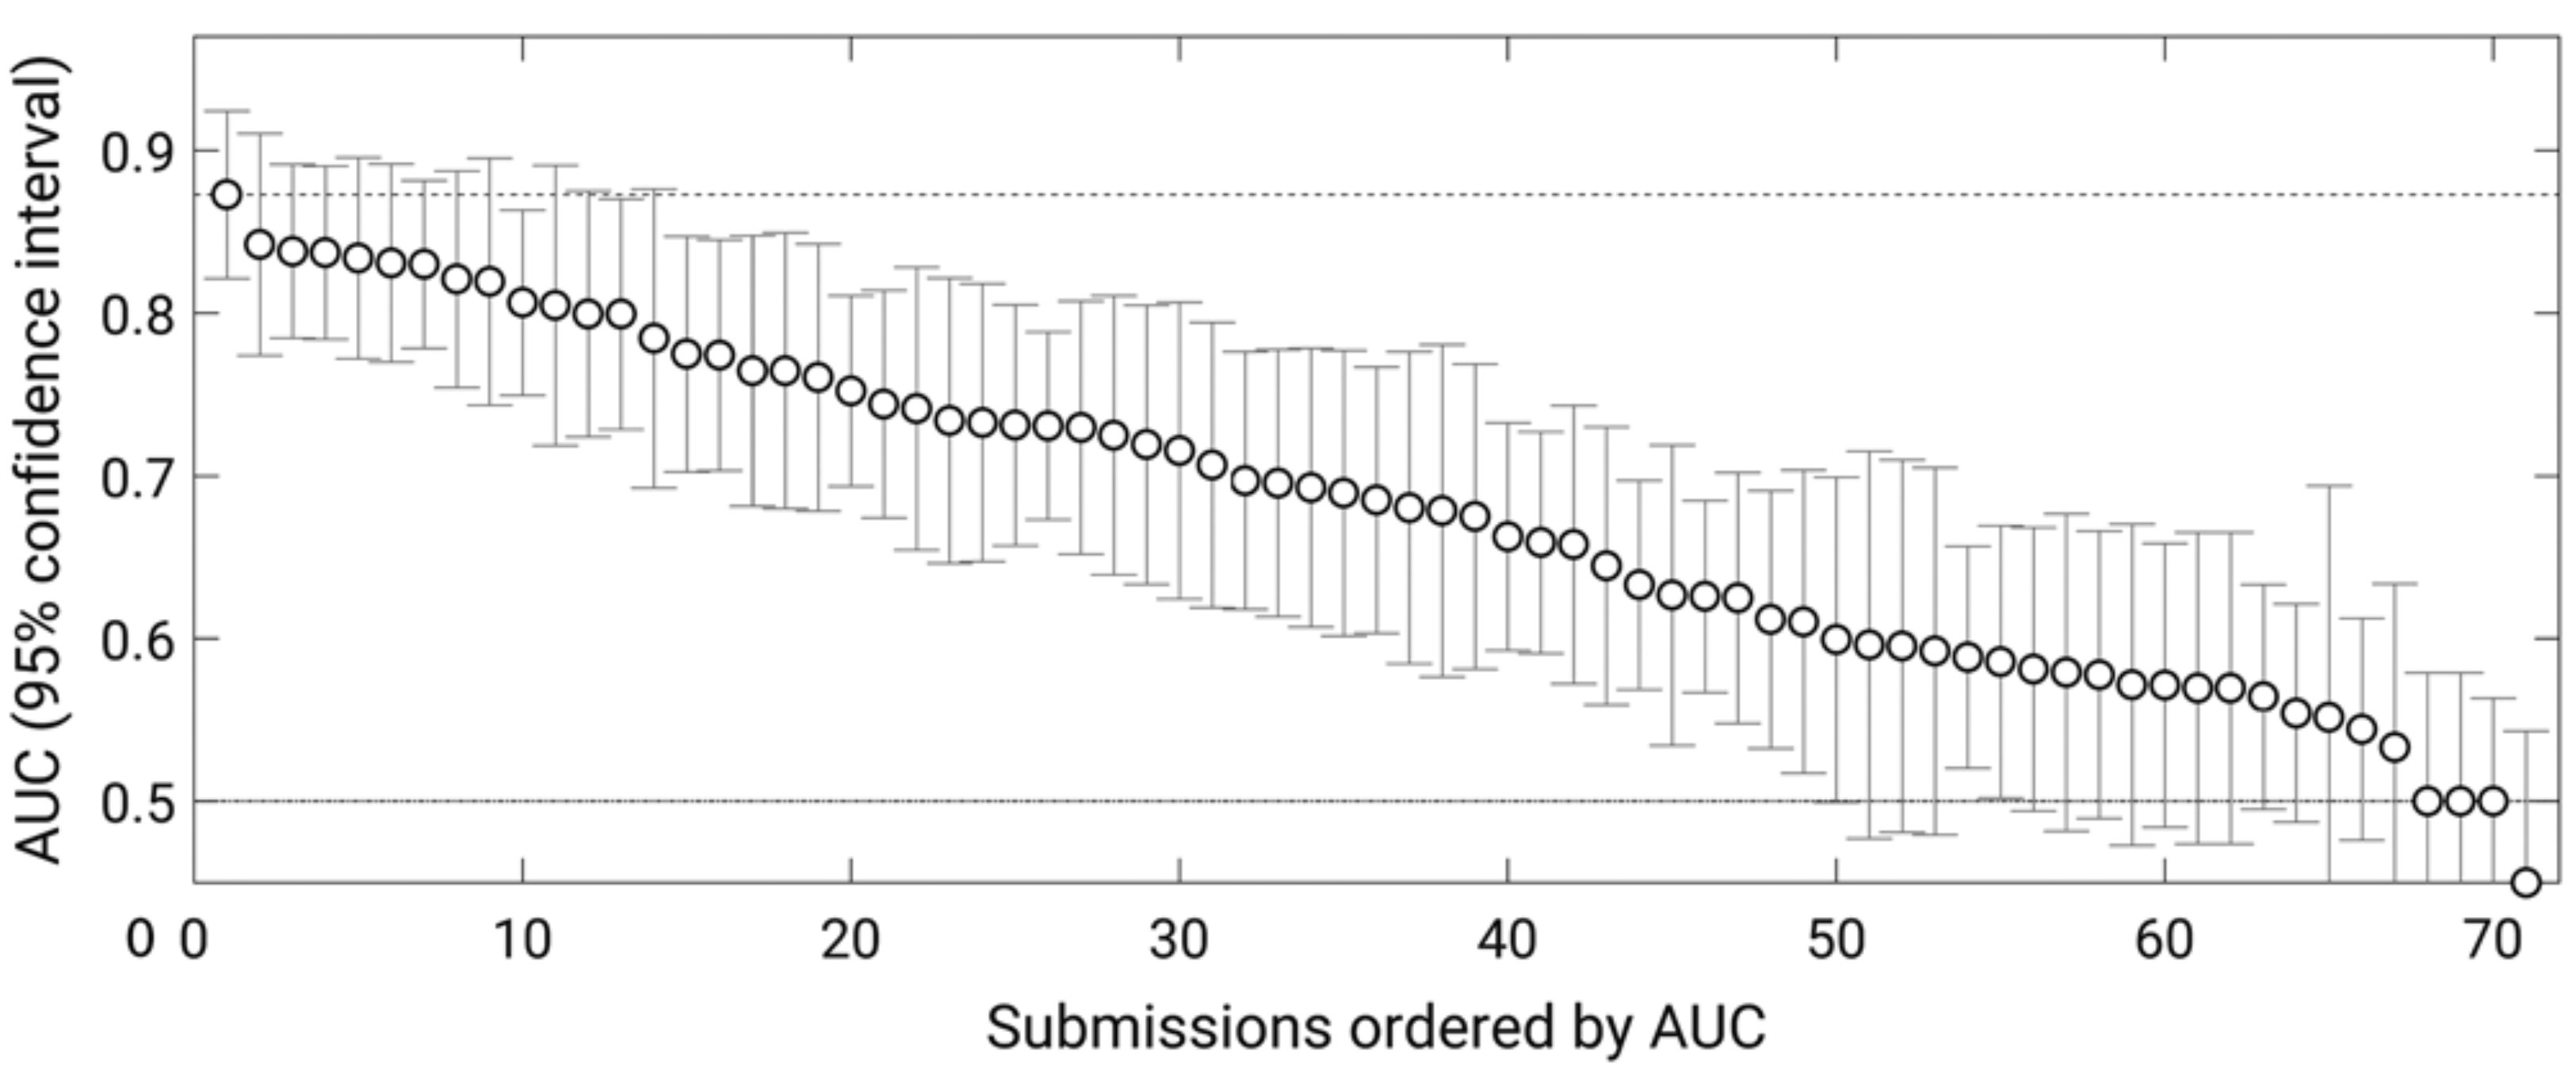
\includegraphics[width=1\textwidth, keepaspectratio=true]{./figures/challenge_all_results.png}
\caption{AUC values achieved by the 71 methods that participated in the PROSTATEx Challenge }
\label{fig:challenge_all_results}
\end{figure}


\section{Lung/Lung CT Challenge}
"Lung cancer is one of the most frequent and leading causes to death all over the world. It was reported that there were approximately $1.8x10^6$ new cases of lung cancer globally in 2012. Early detection of lung cancer, which is typically viewed in the form of lung nodules, is an efficient way to improve the survival rate"\cite{41}. All the articles cited below make use of the SPIE-AAPM Lung CT Challenge dataset, which is a dataset of CT scans devoted to the classification of lung nodules (see \ref{sec:lungCTChallenge} for more details).

Cengil et al. \cite{02} built a fairly simple convolutional neural network to classify images of the Lung CT Challenge dataset. The model takes 4-dimensional data as input (depth, height, width and channels) and performs 3D convolutions on it. The model consists of an input layer, five layers of 3D convolutions (the first is associated with a RELU activation function and pooling, the last with nothing, and the others with pooling) and a fully connected layer at the end. Regarding the model evaluation, authors announce an accuracy of 0.7 on their test set, composed of 30 findings.\\
Armato et al. \cite{12} described the LUNGx Challenge and their results. This challenge consisted in classifying the lung nodules as benign or malignant among a training set of 10 scans and a test set of 60 scans. Since the training set was extremely small, training the model on other datasets was allowed.  The article describes the results of the proposed methods and compare them with the performance of six radiologists on the same task. The article reports that: "ten groups applied their own methods to 73 lung nodules (37 benign and 36 malignant) that were selected to achieve approximate size matching between the two cohorts. Area under the receiver operating characteristic curve (AUC) values for these methods ranged from 0.50 to 0.68. Only three methods performed statistically better than random guessing. The radiologists’ AUC values ranged from 0.70 to 0.85. Three radiologists performed statistically better than the best-performing computer method."\cite{12}. Figure \ref{fig:LUNGx_challenge_all_results} gives an overview of all results.

\begin{figure}[!h]
\centering
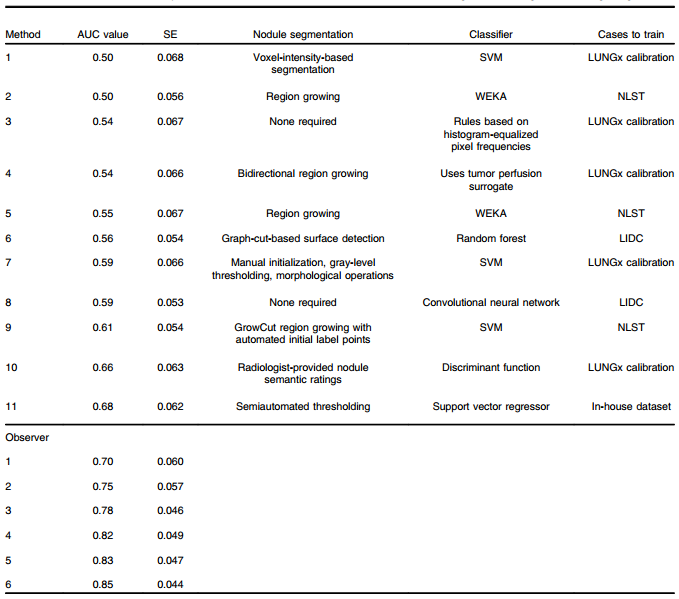
\includegraphics[width=1\textwidth, keepaspectratio=true]{./figures/LUNGx_challenge_all_results.png}
\caption{AUC values for the 11 computerized methods and six radiologists in the task of classifying malignant and benign nodules}
\label{fig:LUNGx_challenge_all_results}
\end{figure}



\section{Brain/Kaggle Brain}
Brain cancer is another major type of cancer. "Brain and other nervous system cancer is the 10th leading cause of death for men and women. It is estimated that 17760 adults (9910 men and 7850 women) will die from primary cancerous brain and central nervous system tumors this year"\cite{43}. All the following articles are based on the Kaggle Brain dataset. This dataset, unlike the ones for the prostate and the lung, does not come from a certified medical authority but from the Kaggle website. However, since it is the only dataset available for the brain tumor classification, some publications used it (see \ref{sec:kaggleBrain} for more details).

Saxena et al. \cite{31} implemented three convolution neural networks to classify the brain tumors coming from the Kaggle "Brain MRI Images for Brain Tumor Detection" dataset. Their processing method used a cropping technique which removed extra black margin around the skull. Each border of the image merges with a part of the skull. Since the images come from different sources, their resolution vary quite a lot. Therefore, the authors resized them to $224x224x3$. Moreover, data was augmented by rotation and vertical/horizontal shifting. As the cropping was performed before augmenting the images, small parts of the brain are outside of the augmented images due to rotation and shifting. The data was split into a training set, a validation set and a test set. Regarding the models, authors implemented three of them (a Resnet-50, a VGG-16 and an Inception-V3) in order to compare their performance. The best results on the test set were achieved by the Resnet-50 (AUC of $0.95$ and accuracy of $0.95$). The VGG-16 was close (AUC of $0.90$ and accuracy of $0.90$), whereas the Inception-V3 didn't perform well (AUC of $0.55$ and accuracy of $0.55$).

%Hanwat et al. \cite{32} implemented a convolutional neural network to classify brain tumors of the Kaggle dataset. Their processing method included skull masking, i.e. the removal of every non-brain tissue from the image. According to the authors, this technique improves performance quite a lot. ---> Check their methods (graphs look special)

Habib Mohamed Ali \cite{04} proposed a self created convolutional neural network to classify the images of the Kaggle Brain dataset. First, the data was augmented. Then, it was cropped to contain only the brain, resized and normalized in order to scale pixel values to the range [0,1]. After the preprocessing, the data was split into a training set (70\%), a validation set (15\%) and a test set (15\%). Regarding the neural network structure, the model is simple. It is composed of only one convolutional layer with a batch norm layer and ReLu activation function, followed by two max pool layers and a dense layer. Thanks to this model, an accuracy of 89\% was achieved on the test set.


% !TEX root = ../main.tex

\chapter{Deep learning}
\label{ch:deep_learning}
This chapter provides the theoretical foundation in deep learning which is required to understand of the rest of the work. It starts with an historical timeline of deep learning before describing what a neural network is. Then, the notion of training a neural network, with all that is involved such as forward propagation, backpropagation, hyperparameters, data splitting or performance evaluation is explained. This part is followed by another section devoted to a special type of neural networks, the "convolutional neural networks". They are used in many computer vision applications due to their great performance for these tasks. Finally, the concept of "transfer learning" is discussed since the entire chapter \ref{ch:transfer_learning} relies on it.


\section{Introduction to deep learning}
Deep learning is currently one of the trendiest topics in machine learning, a subset of artificial intelligence. Machine learning refers to statistical models that allow computers to perform specific tasks without having been explicitly programmed to solve them. In fact, these models try to find structural patterns within data in order to understand new incoming situations and react in the best possible way. There exist various techniques in machine learning such as k-NN, SVM, k-means, decision trees, association rules, etc. What mainly differentiates deep learning from these algorithms is the concept of neural networks (see section  \ref{what_is_a_neural_network}) that are combined to form deep neural networks.\\
Neural networks are inspired from the biological neural networks of the brain. These systems try to learn how to solve a problem based on the data they receive as input. Many concrete applications make use of neural networks: autonomous vehicles, smarter translators, computer-aided diagnoses, personal assistants, art creation, robotics, etc. The presence of deep learning techniques in these use cases clearly testifies to the enthusiasm of many areas for this technology. Furthermore, since this field has recently gained interest (see section \ref{historical_background}), a lot of research is still ongoing, which suggests that many exciting new applications will certainly be discovered in the near future.

\subsection{Historical background}
\label{historical_background}
As described on figure \ref{history}, the theoretical foundations of deep learning appeared long before the invention of computers. From the first attempts to understand the human brain until today, huge progress was made to be establish the basic components of modern neural networks. One could ask why deep learning took off recently if the theory was around for a long time.\\
As stated by Goodfellow et al. \cite{15}, the first part of the answer is computing power. In fact, deep learning algorithms need a lot of data to work properly, which requires powerful CPUs/GPUs that either didn't exist or were only within few people's reach. One other main reason concerns the lack of data. Since deep learning algorithms "learn" from data, learning is impossible if good-quality data are not available. The era of Big Data enhanced deep learning possibilities. 
%%%% Je mettrais soit l'un soit l'autre. Le paragraphe du dessus c'est le paragraphe du dessous avec des autres mots :)
% These two points are summarised: "The increase in model size overtime, due to the availability of faster CPUs, the advent of general purpose GPUs, fasternetwork, connectivity and better software infrastructure for distributed computing, is one of the most important trends in the history of deep learning. This trend is generally expected to continue well into the future".\\
Finally, before the year 2012, the abilities of neural networks were still to be proven. This changed with the ImageNet Large Scale Visual Recognition Challenge (a competition where researchers evaluate their algorithms on several visual recognition tasks). In fact, the deep convolutional neural network called "AlexNet" achieved 16\% of classification error rate, whereas the previous best scores were around 25\%. This victory marked the beginning of a new craze for these types of algorithms.


\begin{figure}[!h]
\centering
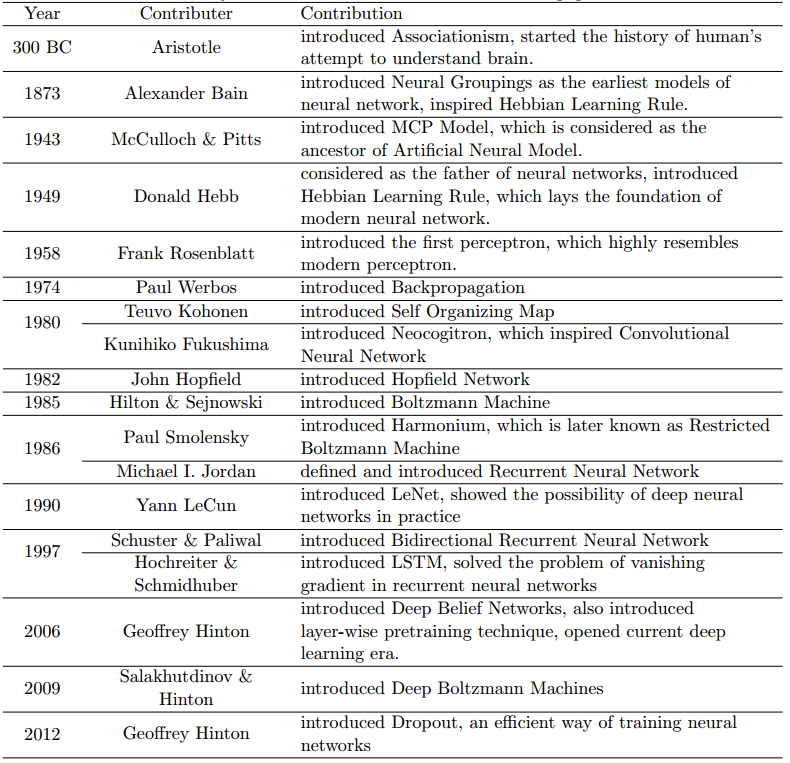
\includegraphics[width=1\textwidth, keepaspectratio=true]{./figures/history.png}
\caption{Deep learning milestones - Wang et al. \cite{14}}
\label{history}
\end{figure}

 
\subsection{What is a neural network?}
\label{what_is_a_neural_network}

From a descriptive point of view, neural networks can simply be seen as a non-linear applications that associate an input to an output with respect to certain parameters. The input can be an image, a sound or any input that can be converted into numerical features. The output of a neural network depends on the problem it tries to solve. In computer vision, the most common types of outputs are classes (for classification problems) and pixel coordinates (for segmentation problems).\\
From a mathematical standpoint, a neural network can be defined as a non-linear function $f$ that associates to an input $x$ an output $y$ with respect to parameters $\theta$.
\begin{equation}
y = f(x,\theta)
\end{equation}
The parameters $\theta$ are estimated from the training samples.
%\begin{figure}[!h]
%\centering
%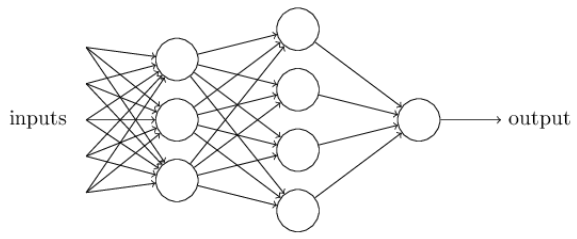
\includegraphics[width=1\textwidth, keepaspectratio=true]{./figures/neural_network.png}
%\caption{Neural Network example}
%\label{neural_network}
%\end{figure}

\subsection{Supervised and unsupervised learning}
In machine learning, two different kinds of tasks exist. The first one is "supervised learning". It includes learning algorithms whose training samples are associated to their labels in order to find the optimal mapping between the input and the output. The second one is "unsupervised learning". In contrast to supervised algorithms, the latter rely on unlabeled data. Its main goal is to infer the natural structure  present in the data. Since the models presented in this work belong to the "supervised learning" category, notions explained below refer to this kind of algorithms.


\section{Neural networks basics}

\subsection{Notation}
In order to keep the mathematical description of neural network consistent, this work will use Andrew Y. Ng's notation \cite{16}, who was a pioneer in deep learning.\\

\noindent \textbf{General comment}
\begin{itemize}
\item Superscript (i) denotes the $i^{th}$ training example.
\item Superscript [l] denotes the $l^{th}$ layer of the neural network.
\end{itemize}

\noindent \textbf{Sizes}
\begin{itemize}
\item $m$: number of examples in the dataset
\item $n_{x}$: input size
\item $n_{y}$: output size (or number of classes)
\item $n_{h}^{[l]}$: number of hidden units (i.e neurons) of the $l^{th}$ layer
\item $L$: number of layers in the network
\end{itemize}

\noindent \textbf{Neural networks components}
\begin{itemize}
\item $X\in \R$ is the input matrix matrix of a neural network.
\item $x^{(i)} \in \R^{n_{x}}$ is the $i^{th}$ example (sample) represented as a column vector.
\item $Y \in \R^{n_{y} \times m}$ is the label matrix.
\item $y^{(i) \in \R^{n_{y}}}$ is the output label for the $i^{th}$ example.
\item $W^{[l]} \in \R$ \textsuperscript{\# of neurons in the next layer = j  x \# of neurons in the previous layer = k} is the weight matrix at layer $[l]$.
\item $b^{[l]} \in R$\textsuperscript{\# of units in next layer} is the bias vector in the $l^{th}$ layer.
\item $\hat{y} \in R^{n_{y}}$ is the predicted output vector. It can also be denoted $a^{[L]}$ where $L$ is the number of layers in the whole network.
\item $g^{[l]}(x)$ is the $l^{th}$ activation function.  
\item $z^{[l]} = W_{x}x^{(i)} + b^{[l]}$ denotes the weighted sum of the input given to the $l^{th}$ layer before passing through the activation function.\\
\end{itemize}

\noindent \textbf{Forward propagation equations}
\begin{itemize}
\item $a = g^{[l]}(W_{x}x^{(i)} + b^{[l]}) = g^{[l]}(z^{[l]})$ where $g^{[l]}$ denotes the $l^{th}$ layer activation function.
\item $a_{j}^{[l]} = g^{[l]} (\sum_{k} w_{jk}^{[l]}a_{k}^{[l-1]} + b_{j}^{[l]}) = g^{[l]} (z_{j}^{[l]}) $ is the general activation formula at $l^{th}$ layer.
\item $J(x, W, b, y)$ and $J(\hat{y}, y)$ denote the cost function.
\end{itemize}

\subsection{Perceptrons}
\label{perceptron}
Perceptrons are the main components of neural networks. They were "developed in the 1950s and 1960s by the scientist Frank Rosenblatt, inspired by earlier work by Warren McCulloch and Walter Pitts" \cite{13}. Today, they are called "artificial neurons" or simply "neurons".\\
A perceptron $j$ is a function $f$ of input $x=(x_{1}, ..., x_{n})$ weighted by a vector of weights $w_{}=(w_{1}, ..., w_{n})$, completed by a bias $b_{j}$ and associated to a non-linear activation function $g$:
\begin{equation}
\label{perceptron_equation}
a_{j} = f_{j}(x) = g((\sum_{k=1}^{n} x_{k} * w_{k}) + b_{})
\end{equation}

Schematically speaking, a perceptron can be represented as on figure \ref{perceptron_model}. Each input is multiplied with its corresponding weight. The sum of this result then goes through a non-linear function, called "activation function". This activation function acts like a threshold that determines the proportion of the result that goes further in the network. There exist multiple activation functions (see \ref{activation_functions}). It is extremely important to use non-linear functions instead of a linear functions. In fact, the output of a perceptron is given as input to the others (see \ref{multilayer_perceptron}). Consequently, if linear functions only are used throughout the network, linear outputs are given as inputs to other linear functions. Since the composition of two linear functions is itself a linear function, assembling perceptrons to create neural networks of multiple layers would not make sense anymore.


\tikzset{basic/.style={draw,fill=white!20,text width=1em,text badly centered}}
\tikzset{input/.style={basic,circle}}
\tikzset{weights/.style={basic,rectangle}}
\tikzset{functions/.style={basic,circle,fill=white!10}}



\begin{figure}[!h]
\centering
	\begin{tikzpicture}
	
	\node[functions] (center) {};
        \node[below of=center,font=\scriptsize,text width=4em] {Activation function};
        \draw[thick] (0.5em,0.5em) -- (0,0.5em) -- (0,-0.5em) -- (-0.5em,-0.5em);
        \draw (0em,0.75em) -- (0em,-0.75em);
        \draw (0.75em,0em) -- (-0.75em,0em);
        \node[right of=center] (right) {};
            \path[draw,->] (center) -- (right);
        \node[functions,left=5em] (left) {$\sum$};
            \path[draw,->] (left) -- (center);
        \node[weights,left=15em] (2) {$w_2$} -- (2) node[input,left of=2] (l2) {$x_2$};
            \path[draw,->] (l2) -- (2);
            \path[draw,->] (2) -- (left);
        \node[below of=2] (dots) {$\vdots$} -- (dots) node[left of=dots] (ldots) {$\vdots$};
        \node[weights,below of=dots] (n) {$w_n$} -- (n) node[input,left of=n] (ln) {$x_n$};
            \path[draw,->] (ln) -- (n);
            \path[draw,->] (n) -- (left);
        \node[weights,above of=2] (1) {$w_1$} -- (1) node[input,left of=1] (l1) {$x_1$};
            \path[draw,->] (l1) -- (1);
            \path[draw,->] (1) -- (left);
        \node[weights,above of=1] (0) {$w_0$} -- (0) node[input,left of=0] (l0) {$1$};
            \path[draw,->] (l0) -- (0);
            \path[draw,->] (0) -- (left);
        \node[below of=ln,font=\scriptsize] {inputs};
        \node[below of=n,font=\scriptsize] {weights};
	
	\end{tikzpicture}
\caption{The perceptron model}
\label{perceptron_model}
\end{figure}

\subsection{Activation functions}
\label{activation_functions}
Once the computation of the weighted sum of all inputs for a specific neuron is done, the latter has to pass the sum through an activation function that will decide the proportion of the result that will be sent to the next layer. Activation functions must be non-linear in order to approximate extremely complex functions. In fact, neural networks are considered as universal approximators. Hornik et al. claim that "multilayer feedforward networks are capable of approximating any measurable function to any desired degree of accuracy, in a very specific and satisfying sense" \cite{17}. According to Thomas Epelbaum \cite{18}, the most commonly used activation functions are:\\\\
 \noindent \textbf{Sigmoid function}\\
 The sigmoid function is defined as:
 \begin{equation}
  g(x) = \frac{1}{1+e^{-x}}
 \end{equation}
 Its derivative is:
 \begin{equation}
 g'(x) = g(x)(1-g(x))
 \end{equation}
 


\begin{figure}[h!]
  \begin{center}
    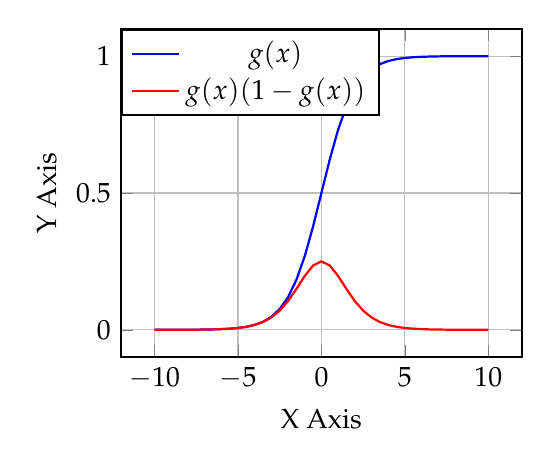
\begin{tikzpicture}
      \begin{axis}[
      	  width=0.55\linewidth, % Scale the plot to 0.7 \linewidth
          xlabel={$x$}, 
          ylabel={$y$},
          xlabel=X Axis, 
          ylabel=Y Axis,
          samples=41, 
          grid, 
          thick,
          domain=-10:10,
		legend style={at={(0,1)},anchor=north west}
        ]
        \addplot+[no marks] {1/(1+exp(-x))};
        \addlegendentry{$g(x)$}
        \addplot+[no marks] {(1/(1+exp(-x))) * (1-(1/(1+exp(-x))))};
        \addlegendentry{$g(x)(1-g(x))$}
      \end{axis}
    \end{tikzpicture}
    \caption{The sigmoid function and its derivative}
  \end{center}
\end{figure} 
 
 
 \noindent \textbf{Tanh function}\\
 \begin{equation}
 g(x) = tanh(x) = \frac{1-e^{-2x}}{1+e^{-2x}}
 \end{equation}
 Its derivative is:
 \begin{equation}
 g'(x) = tanh'(x) = 1-tanh^{2}(x)
 \end{equation}
 
  \begin{figure}[h!]
  \begin{center}
    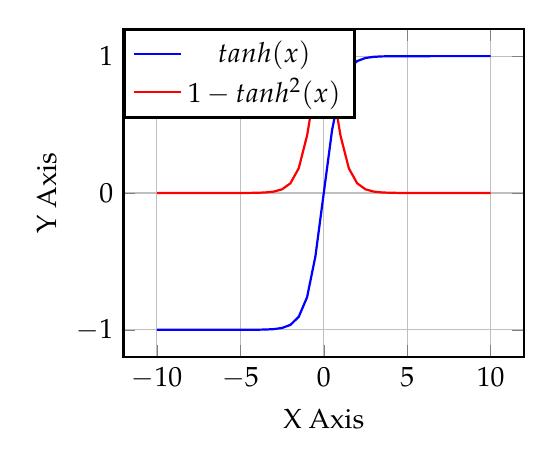
\begin{tikzpicture}
      \begin{axis}[
      	  width=0.55\linewidth, % Scale the plot to 0.7 \linewidth
          xlabel={$x$}, 
          ylabel={$y$},
          xlabel=X Axis, 
          ylabel=Y Axis,
          samples=41, 
          grid, 
          thick,
          domain=-10:10,
		legend style={at={(0,1)},anchor=north west}
        ]
        \addplot+[no marks] {(1-exp(-2*x))/(1+exp(-2*x))};
        \addlegendentry{$tanh(x)$}
        \addplot+[no marks] {1-((1-exp(-2*x))/(1+exp(-2*x)))^2};
        \addlegendentry{$1-tanh^{2}(x)$}
      \end{axis}
    \end{tikzpicture}
    \caption{The tanh function and its derivative}
  \end{center}
\end{figure} 
 
 \noindent \textbf{ReLU function}\\
 \begin{equation}
 g(x) = ReLU(x) = 
 \begin{cases}
    1 & \text{if } x\geq 0\\
    0              & \text{otherwise}
\end{cases}
 \end{equation}
 
 \begin{figure}[h!]
  \begin{center}
    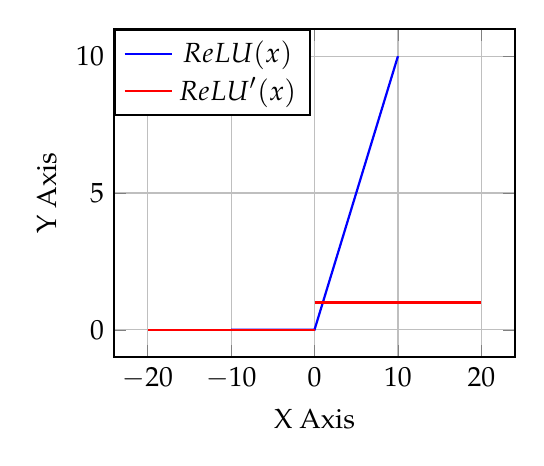
\begin{tikzpicture}[
    declare function={
    func(\x)= (\x<=0) * (0);
  }
  ]
      \begin{axis}[
      	  width=0.55\linewidth, % Scale the plot to 0.7 \linewidth
          xlabel={$x$}, 
          ylabel={$y$},
          xlabel=X Axis, 
          ylabel=Y Axis,
          samples=41, 
          grid, 
          thick,
          domain=-10:10,
		legend style={at={(0,1)},anchor=north west}
        ]
        \addplot+[no marks] {(x>=0)*x};
        \addlegendentry{$ReLU(x)$}
        \addplot[domain=-20:0,red] {0};
		\addplot[domain=0:20, red] {1};
        \addlegendentry{$ReLU'(x)$}
      \end{axis}
    \end{tikzpicture}
    \caption{The ReLU function and its derivative (undefined when $x=0$)}
  \end{center}
\end{figure} 
 
 
 
 
 \noindent \textbf{ELU function}\\
 \begin{equation}
 g(x) = 
 \begin{cases}
    x & \text{if } x\geq 0\\
    e^{x}-1 & \text{otherwise }
\end{cases}
 \end{equation}
 Its derivative is:
 \begin{equation}
g'(x) = 
 \begin{cases}
    1 & \text{if } x\geq 0\\
    e^{x} & \text{otherwise }
\end{cases}
 \end{equation}
 
 

  \begin{figure}[h!]
  \begin{center}
    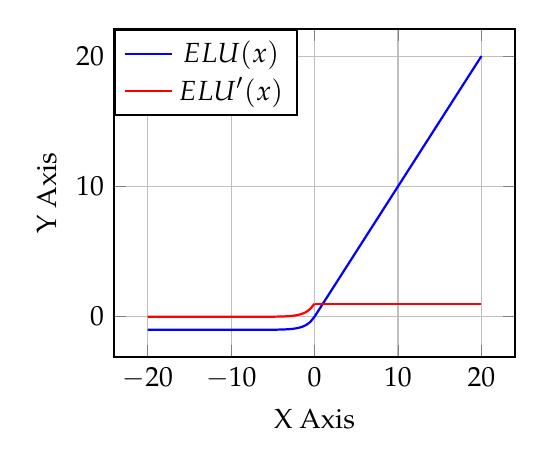
\begin{tikzpicture}[
    declare function={
    func(\x)= (\x>=0) * (x) +and (\x<0) * 4;
  }
    ]
      \begin{axis}[
      	  width=0.55\linewidth, % Scale the plot to 0.7 \linewidth
          xlabel={$x$}, 
          ylabel={$y$},
          xlabel=X Axis, 
          ylabel=Y Axis,
          samples=41, 
          grid, 
          thick,
          domain=-10:10,
		legend style={at={(0,1)},anchor=north west}
        ]
        \addplot[domain=0:20, blue] {x};
        \addlegendentry{$ELU(x)$}
        \addplot[domain=0:20,red] {1};
        \addlegendentry{$ELU'(x)$}
          
        \addplot[domain=-20:0,red] {exp(x)};
        \addplot[domain=-20:0,blue] {exp(x)-1};
        
      \end{axis}
    \end{tikzpicture}
    \caption{The ELU function and its derivative}
  \end{center}
\end{figure} 

\subsection{Multilayer perceptrons}
\label{multilayer_perceptron}
A multilayer perceptron is a type of artifical neural networks. Du et al. \cite{23} define multilayer perceptrons as "feedforward networks with one or more layers of units between the
input and output layers" where "the output units represent a hyperplane in the space
of the input patterns."\\
A multilayer perceptron is composed of $L$ layers, each of them composed of $n^{l}_{h}$ perceptrons. The layers are organized in the following way:
\begin{itemize}
\item The input layer: it is the neural network entry point for the data. Generally speaking, the data is provided in the form of a matrix $X \in \R$ of size $(n_{x} \times batch\_size)$ with their corresponding labels $Y \in \R$ of size $(n_{y} \times batch\_size)$. The batch size defines the number of samples that will be given at the same time to the network and $n_{x}$ is the dimension of each sample. Moreover, $x^{(i)}$ is the $i^{th}$ sample represented as a column vector. The total number of training samples is given by $m$. Finally, $y^{(i)}$ is the output label for the $i^{th}$ example. For instance, suppose the number of samples is 100 and the batch size 32. In this situation, the network will be feeded with 4 batches of sizes [32, 32, 32, 4] respectively. 

\item The hidden layer(s): hidden layers stand for all layers that are between the input layer and the output layer. Each of them has its own weights and biases (W, b), denoted by $W^{[l]} \in \R $ and $b^{[l]}$ respectively, where $W_{ij}^{l}$ corresponds to the weights associated with the connection between perceptron $j$ in layer $l$ and perceptron $i$ in layer $l+1$. By analogy, $b_{i}^{[l]}$ is the bias associated with perceptron $i$ in layer $l$. Weights and biases are the parameters to optimize in order to obtain the best mapping between the input and the output of the network (see section \ref{training_a_neural_network} ). Before training the neural network, the weights can be randomly initialized or initialized with more sophisticated methods such as "Xavier initialization" or "Kaiming initialization"(see section \ref{weight_initialization}).

\item The output layer: it is the last layer of the neural network. Its role is essential since it produces the prediction of the network for a given input. The prediction of a neural network is given by $\hat{y} \in R^{n_{y}}$ with $n_{y}$ beeing the number of different labels. In a classification task, whose goal is to assign to each input a specific class, the $\hat{y}$ is usually the probability that the input belongs to each class. In that case, the \textit{softmax} activation function would be used at the end.
\end{itemize}
The advantage of organizing the weights, biases and inputs in matrices is due to the ability of modern CPUs/GPUs to quickly perform linear algebra computations. This way of structuring the network component is called "vectorization" which avoids using loops in the code, which would considerably slow down the computations.
Figure \ref{multilayer_perceptrons_figure} illustrates the concept of multilayer perceptrons. In this example, the total number of layers $L$ is equal to 3, the input size $n_{x}$ is equal to 4 and the number of units in in each layer is $n_{h}^{1}= 4$, $n_{h}^{2}=2$, $n_{h}^{3}=1$. The network contains the weights  $W^{(1)} \in \R^{2x3}$, $W^{(2)} \in \R^{1x2}$ and the biases  $b^{[1]}=2$, $b^{[2]}=1$.


\begin{figure}[!h]
\centering
	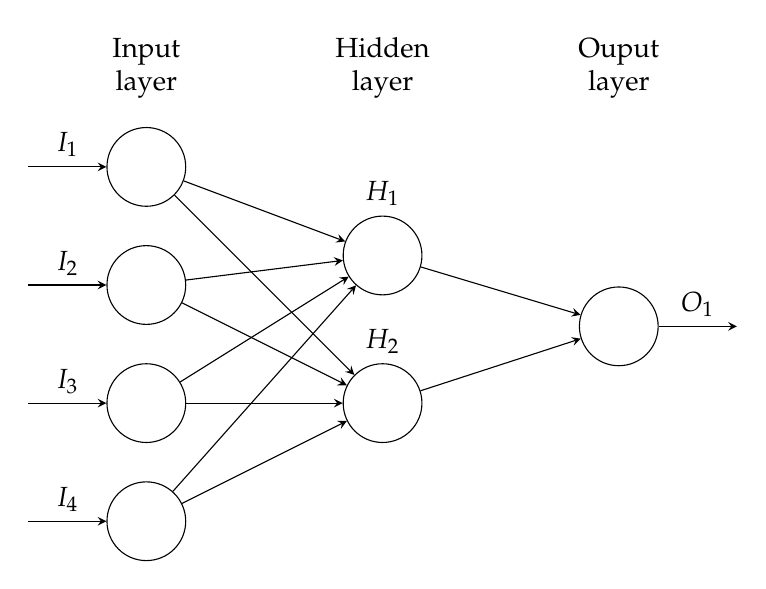
\begin{tikzpicture}[x=1.5cm, y=1.5cm, >=stealth]
	
	\foreach \m/\l [count=\y] in {1,2,3,4}
	  \node [every neuron/.try, neuron \m/.try] (input-\m) at (0,2.5-\y) {};
	
	\foreach \m [count=\y] in {1,2}
	  \node [every neuron/.try, neuron \m/.try ] (hidden-\m) at (2,2-\y*1.25) {};
	
	\foreach \m [count=\y] in {1}
	  \node [every neuron/.try, neuron \m/.try ] (output-\m) at (4,0.15) {};
	
	% input layer
	\foreach \l [count=\i] in {1,2,3,4}
	  \draw [<-] (input-\i) -- ++(-1,0)
	    node [above, midway] {$I_\l$};
	
	% hidden layer
	\foreach \l [count=\i] in {1,2}
	  \node [above] at (hidden-\i.north) {$H_\l$};
	
	% output neurons
	\foreach \l [count=\i] in {1}
	  \draw [->] (output-\i) -- ++(1,0)
	    node [above, midway] {$O_\l$};
	
	% input -> hidden
	\foreach \i in {1,...,4}
	  \foreach \j in {1,...,2}
	    \draw [->] (input-\i) -- (hidden-\j);
	
	% hidden -> output
	\foreach \i in {1,...,2}
	  \foreach \j in {1}
	    \draw [->] (hidden-\i) -- (output-\j);
	
	% labels above layers
	\foreach \l [count=\x from 0] in {Input, Hidden, Ouput}
	  \node [align=center, above] at (\x*2,2) {\l \\ layer};
	
	\end{tikzpicture}
\caption{Multilayer perceptrons}
\label{multilayer_perceptrons_figure}
\end{figure}

\section{Training a neural network}
\label{training_a_neural_network}
Training a neural network can be broken down into multiple steps. The first one is the "forward propagation" step. It consists in giving examples that need to be classified (or segmented, depending on the task) to the untrained neural network and to spread intermediate results through all layers of the network. %Passing all batches as input to a network is called an "epoch". 
After seeing every single batch, the loss is computed using a "loss function". The latter is used to evaluate the predictions of the neural network in comparison to their ground-truth. Then, the weights and biases of the networks are updated during a process called "backpropagation" in order find the global minimum of the loss function. As soon as the neural network has seen every single batch, the end of an "epoch" is reached. This process is repeated for a defined number of epochs.


\subsection{Forward propagation}
The forward propagation is used to transmit the input through the entire neural network. Mathematically speaking, the forward propagation step for a specific layer $l$ is represented by two equations. The first equation denotes the weighted sum of the input given to the $l^{th}$ layer before passing through the activation function $g$: 
\begin{equation}
z^{[l]} = W_{x}^{[l]}x^{(i)} + b^{[l]}
\end{equation}
The second equation describes the effect of the activation function:
\begin{equation}
a^{[l]} = g^{[l]}(z^{[l]})
\end{equation}
Since the output of the activation function is then given as input to all the neurons of the next layer, the whole forward propagation step can be defined as:
\begin{equation}
a_{j}^{[l]} = g^{[l]} (\sum_{k} w_{jk}^{[l]}a_{k}^{[l-1]} + b_{j}^{[l]}) = g^{[l]} (z_{j}^{[l]}) 
\end{equation}
Figure \ref{forward_propagation} illustrates the computation of the forward propagation pass for the $l^{th}$ layer. The weight natrix $W_{jk}^{l}$ represents the weights associated with the connection between perceptron $k$ in layer $l$ and perceptron $j$ in layer $l+1$. This matrix is multiplied by the output of the previous layer $a_{j}^{[l-1]}$ before adding the bias $b^{[l]}$. The result is given as input to the activation function.

\begin{figure}[!h]
\centering
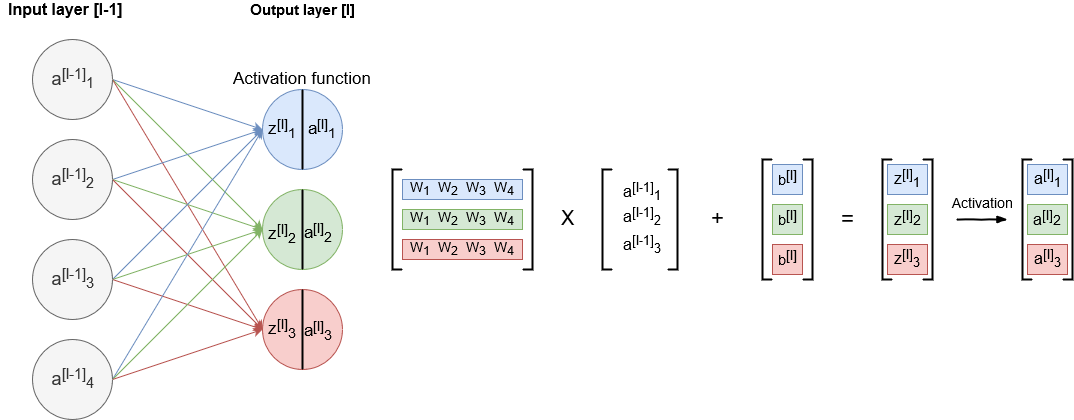
\includegraphics[width=1\textwidth, keepaspectratio=true]{./figures/forward_propagation.png}
\caption{Forward propagation }
\label{forward_propagation}
\end{figure}

\subsection{Loss computation}
As stated by Thomas Epelbaum, "the loss function evaluates the error performed by the neural network when it tries to estimate the data to be predicted" \cite{18}. It is therefore useful to measure the penalty for a single input. On the contrary, when the goal is to get a more general overview of the error on the entire batch or on the entire dataset, the cost function $J$ is used. The latter is represented by $J(\hat{y}, y)$ where $\hat{y}$ is the prediction of the neural network and $y$ the real label. 

There exist multiple cost functions. For a regression problem, a commonly used loss function is the mean square error:
\begin{equation}
J(\hat{y}, y) = \frac{1}{m}[\sum_{i=1}^{m} (\hat{y}^{(i)} - y^{(i)})^{2}]
\end{equation}
For classification problems, the cross entropy function is regularly used. We distinguish the binary classification where the number of classes $n_{y}$ = 2 from the multiclass classification where $n_{y}$ > 2. In the case of binary classification, the cross entropy is:
\begin{equation}
J(\hat{y}, y) = -\frac{1}{m}\sum_{i=1}^{m} [y_{i}*log(\hat{y}_{i}) + (1-y_{i})*log(1-\hat{y_i})]
\end{equation}
In the case of multiclass classification, the categorical crossentropy is:
\begin{equation}
J(\hat{y}, y) = - \sum_{i=1}^{n_{y}} \sum_{j=1}^{m} (y_{ij}*log(\hat{y}_{ij}))
\end{equation}

Since the cost function gives an estimation of the overall error of the network, the main objective of training a neural network is to update its weights in order to approach the minimum of the function. Therefore, deep learning problems can be considered as optimization problems. Solutions to these problems can be found using the gradient descent algorithm during backpropagation.

\subsection{Backpropagation}
Backpropagation relies on a technique called "gradient descent" to minimize the cost function $J(W, b)$. Generally speaking, "the intuition behind the backpropagation algorithm is as follows. Given a training example $(x^{(i)}, y^{(i)})$, we will first run a forward pass to compute all the activations throughout the network, including the output value of the network. Then, for each node $i$ in layer $l$, we would like to compute an "error term" $\partial^{(l)}_{i}$ that measures how much that node was "responsible" for any errors in our output. For an output node, we can directly measure the difference between the network’s activation and the true target value, and use that to define $\partial^{(n_{l})}_{i}$(where layer $n_{l}$ is the output layer). How about hidden units? For those, we will compute $\delta^{(l)}_{i}$ based on a weighted average of the error terms of the nodes that uses $a^{(l)}_{i}$ as an input" \cite{24}.

In other words, after each forward pass through the entire network, backpropagation performs a backward pass which aims at minimizing the cost function by adjusting parameters of the model. The way parameters are updated is defined by the gradients of the cost function with respect to each parameter of the network. The gradient of the cost function $J(x_{1}, x_{2}, ..., x_{m})$ at point $x$ is given by:
\begin{equation}
\frac{\partial J}{\partial x} = [\frac{\partial J}{\partial x_{1}}, \frac{\partial J}{\partial x_{2}}, ..., \frac{\partial J}{\partial x_{1}}]
\end{equation}
The gradient shows how much all parameters that constitute x need to change to minimize the function. In neural networks, the parameters of the cost function are all weight matrices $W^{[l]}$ and biases $b^{[l]}$. The computation of all these gradients relies on the "chain rule". Inthe case of weights, the chain rule is:
\begin{equation}
\frac{\partial J}{\partial w_{jk}^{l}} = \frac{\partial J}{\partial z_{j}^{l}} * \frac{\partial z_{j}^{l}}{\partial w_{jk}^{l}}
\end{equation}
Similarly, the chain rules has to be applied to the biases:
\begin{equation}
\frac{\partial J}{\partial b_{j}^{l}} = \frac{\partial J}{\partial z_{j}^{l}} * \frac{\partial z_{j}^{l}}{\partial b_{j}^{l}}
\end{equation}
Once the gradients of each parameter are computed, these parameters are updated. The weights update is described by the following equation:
\begin{equation}
W^{[l]} = W^{[l]} - \alpha * \frac{\partial J}{\partial W^{[l]}}
\end{equation}
The biases update corresponds to:
\begin{equation}
b^{[l]} = b^{[l]} - \alpha * \frac{\partial J}{\partial b^{[l]}}
\end{equation}
%The hyperparameter $\alpha$ of these two equations is called "learning rate". It determines the gradient's influence at each epoch and has to be manually tuned.
The "learning rate" $\alpha$ determines the influence that the gradient has at each epoch. It is an hyperparameter and has to be tuned manually.


\subsection{Metrics}
In classification tasks, four separate output labels can occur:
\begin{itemize}
\item True Positive (TP):  an output belongs to this class if the prediction that the latter \textbf{contains} a certain feature is \textbf{correct}.
\item True Negative (TN): an output belongs to this class if the prediction that the latter does \textbf{not contain} a certain feature is \textbf{correct}.
\item False Positive (FP): an output belongs to this class if the prediction that the latter \textbf{contains} a certain feature is \textbf{incorrect}.
\item False Negative (FN): an output belongs to this class if the prediction that the latter does \textbf{not contain} a certain feature is \textbf{incorrect}.
\end{itemize}
From these four categories, multiple metrics with their own specificities can be computed \cite{25}:
\begin{itemize}
\item Accuracy: ratio of the correctly labeled subjects to the whole pool of subjects.
\begin{equation}
Accuracy = \frac{(TP+TN)}{TP+FP+FN+TN}
\end{equation}
Accuracy is a great measure in the case of symmetric data (i.e the number of FN $\approx$ FP and their cost is similar). When this condition is not fulfilled, accuracy can lead to bad models. For instance, let's define a binary classification model that always outputs class 0. If the data is composed of 99 samples from class 0 and 1 sample from class 1, the accuracy is equal to 99\% but the model is not smart. Consequently, this metric has to be used in addition to other metrics.

\item Precision: ratio of the correctly positive labeled subjects by the model to all positive labeled subjects.
\begin{equation}
Precision = \frac{TP}{(TP + FP)}
\end{equation}
This metric is recommended when the confidence of the true positives predicted by the model is important. For instance, this happens in spam blockers where it is preferable to have a spam in mailbox rather than a regular mail in the spam box.

\item Recall (sensitivity):
\begin{equation}
Recall = \frac{TP}{(TP + FN)}
\end{equation}
This metric is recommended when the occurence of false negatives is intolerable and false positives are preferred. This makes perfect sense for disease detection models: labeling an healthy person as unhealthy is better than labeling an unhealthy person as healthy.

\item F1-score:
\begin{equation}
F1-score = \frac{2* recall * precision}{(recall + precision)}
\end{equation}
F1-score considers both precision and recall and is the highest if these two metrics are balanced. This metric is perfectly suitable when the cost of false positives and false negatives is not the same.

\item Specificity:
\begin{equation}
Specificity = \frac{TN}{(TN + FP)}
\end{equation}
This metric is recommended when the occurence of false positives is intolerable whereas true negatives are desired. For instance drug tests can not indicate false positives but they have to cover all true negatives.
\item ROC curve and AUC:
As explained by Sarang Narkhede, "The ROC curve is plotted with recall against the false positive rate (1-specificity) where recall is on y-axis and the false positive rate is on the x-axis. AUC - ROC curve is a performance measurement for classification problem at various thresholds settings. ROC is a probability curve and AUC represents degree or measure of separability. It tells how much model is capable of distinguishing between classes. Higher the AUC, better the model is at predicting 0s as 0s and 1s as 1s" \cite{26}.

\end{itemize}




\subsection{Data}
In deep learning, data is essential. As seen previously, neural networks learn features from it. Therefore, data has to be handled carefully and in the right way. Usually, it is split into three different sets:
\begin{itemize}
\item The training set: this is the part of the dataset that is used to train the neural network (the weights and biases).
\item The validation set: this the dataset that is used to evaluate a trained model. Usually, the evaluation on the validation set is performed every $N$ epochs, where $N$ is a fixed number. The validation set needs to come from the same distribution as the training set but should contain exclusively unseen data. This last point is crucial since the validation set shows how well the neural network generalizes on unknown data. The validation set can also be used as indicator to decide when the training should be stopped in order to prevent "overfitting" which is the behaviour of a model that fits to the training set too closely and don't generalize well. In fact, if the validation loss continuously increases for a certain number of epochs, going on with the training will increase the overfit. This fact of interrupting the training earlier is called "early stopping".
\item The test set: this last part of the dataset is used to establish the final evaluation of the model. It also contains unseen data exclusively. 
\end{itemize}
Regarding the way these three sets are split, it mostly depends on the number of samples available. If the latter is big, the data is split into training and testing using the ratio 80/20. Then the remaining training samples are also split into training and validation using the ratio 80/20. On the contrary, if there are few data available, k-fold cross-validation is a good practice. This technique consists in splitting the entire dataset into k folds. One fold is picked as test set and the others are considered as training sets. The model is trained on training folds and tested on the test set. Then, another test set is picked and the same process is repeated until all possible tests set are picked. At the end of the process, the results of all test sets are averaged, which provides a good estimation of the model's performance. This technique is summarized on figure \ref{cross_validation}.

\begin{figure}[!h]
\centering
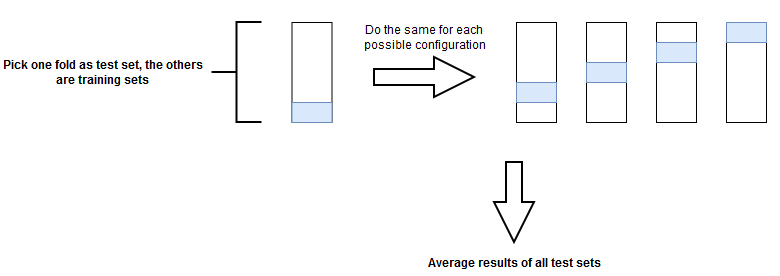
\includegraphics[width=1\textwidth, keepaspectratio=true]{./figures/cross_validation.png}
\caption{5-folds cross-validation }
\label{cross_validation}
\end{figure}


\subsection{Weight initialization}
\label{weight_initialization}
Before training a neural network, the weights have to be initialized in order to proceed to the first forward propagation. The initialization of the neural network weights is crucial since it will determine how quickly the network converges to an optimum. The idea behind weight initialization is to generate an initialization that "prevents layer activation outputs from exploding or vanishing during the course of a forward pass through a deep neural network. If either occurs, loss gradients will either be too large or too small to flow backwards beneficially, and the network will take longer to converge, if it is even able to do so at all" \cite{27}.\\
The simplest and least efficient technique to initialize neural network weights is to randomly generate them. The major problem of this technique comes from the fact that some initializations can lead to extremely small or big values, which lead to value near 0 or 1 for most activation functions. Consequently, the slope of the gradient changes slowly and the learning takes a lot of time.\\
To prevent this effect when the tanh activation function is used, "Xavier initialization" multiplies the random initialization by the fraction:
\begin{equation}
\frac{\sqrt{6}}{\sqrt{n_{h}^{[l]}+n_{h}^{[l+1]}}}
\end{equation}
where $n_{h}^{[l]}$ is the number of incoming network connections to the layer and $n_{h}^{[l+1]}$ is the number of outgoing network connections from that layer.\\
For activation functions that are not symmetric around zero and don't have outputs inside [-1,1] such as ReLU or ELU, Kaiming initialization is an alternative. It consists in multiplying the randomly initialized  weight matrix by:
\begin{equation}
\frac{\sqrt{2}}{\sqrt{n_{h}^{[l]}}}
\end{equation} 
where $n_{h}^{[l]}$ is the number of incoming connections coming into a given layer from the previous layer's output.

\subsection{Hyperparameters tuning}
Hyperparameters denote parameters that cannot be directly learned from the data. That is the case for the learning rate, the batch size and the number of epochs that were described in previous sections. So, these parameters have to be manually tuned in order to find the best configuration (i.e the one that minimizes the cost function and that keeps a acceptable level of generalization).\\
Regarding the learning rate $\alpha$, its value has to be neither too large or too small. A too large learning rate is recognizable by analyzing the training loss curve: if "the loss is exploding or fluctuating" or if "it has stopped improving and it is wandering around a suboptimal local optima" \cite{28}, the learning rate is too high and should be decreased. On the contrary, if "the learning is very slow and the loss is decreasing consistently" or if "the model is overfitting" \cite{28}, it is a clear sign that it should be increased.
The learning rate can take a wide range of values. Consequently, the most used technique to find the optimal learning rate is simply the "trial and error", which consists in "trying widely different learning rates to determine the range of learning rates that need to be explored" \cite{28}. There also exists methods that, instead of keeping a fixed learning rate for the entire training, reduce it after each epoch (learning rate decay) or each time the loss on the validation set does not decrease (learning rate scheduling).\\
Batch size is another important hyperparameter to tune. Training a network with a small batch size "requires less memory, since the latter is trained using fewer samples" \cite{29}. Furthermore, "networks train faster because the weights update is done after each propagation" \cite{29}. Nevertheless, "the smaller the batch the less accurate the estimate of the gradient will be" \cite{29}. Indeed, due to the high weights update frequency, the gradient fluctuates much more than if was computed after a bigger number of samples.\\
Finally, the number of epochs during which the network is trained has to be carefully chosen. In fact, from a certain point in the training, neural networks don't learn anymore useful features in the data and start overfitting. This point corresponds to the moment where, the validation loss does not decrease anymore and starts to increase continuously. It is exactly at this moment that the training should stop. To achieve this goal, it is possible either to directly choose the right number of epochs or to use "early stopping", which stops the training as soon as the validation loss does not decrease for $N$ epochs.



\section{Convolutional Neural Networks}

Convolutional Neural Networks (CNN) are a specific type of deep neural networks. They are particular in that they contain layers which perform a mathematical operation named convolution on the input data. CNNs are mostly used in image and video analysis. 

To perform a convolution, numerical input data and a "filter" are required. A filter can be seen as a an $fxf$ numerical patch that moves across the entire input. It first moves horizontally until reaching the right-most border of the image. Then, it goes down a cell and starts from the border on the left-hand side. This process is repeated until the filter reaches the bottom-right corner of the image, which marks the end of the convolution. At each step, the dot product between the filter and the part of the input covered by the filter is computed. Figure \ref{fig:convolution} showcases a simple convolution which aims at finding vertical lines in a black and white image. For example, the output of the first step of the convolution (in red) is computed by evaluating the dot product between the blue filter and the red part of the input image: 
\begin{equation}
\begin{gathered}
\color{blue}(-1) \color{black}* \color{red}0 \color{black}+ \color{blue}2 \color{black}* \color{red}0 \color{black}+ \color{blue}(-1) \color{black}* \color{red}0
\\ \color{black}+ \\ 
\color{blue}(-1) \color{black}* \color{red}0 \color{black}+ \color{blue}2 \color{black}* \color{red}0 \color{black}+ \color{blue}(-1) \color{black}* \color{red}1 
\\ \color{black}+ \\ 
\color{blue}(-1) \color{black}* \color{red}0 \color{black}+ \color{blue}2 \color{black}* \color{red}0 \color{black}+ \color{blue}(-1) \color{black}* \color{red}1 
\\ \color{black}= -2
\end{gathered}
\end{equation}

\noindent The output of the entire convolution shows negative values in the outside parts and large positive values in the center. This means that the $3x3$ filter detected a vertical line in the center of the input image. 

\begin{figure}[!h]
\centering
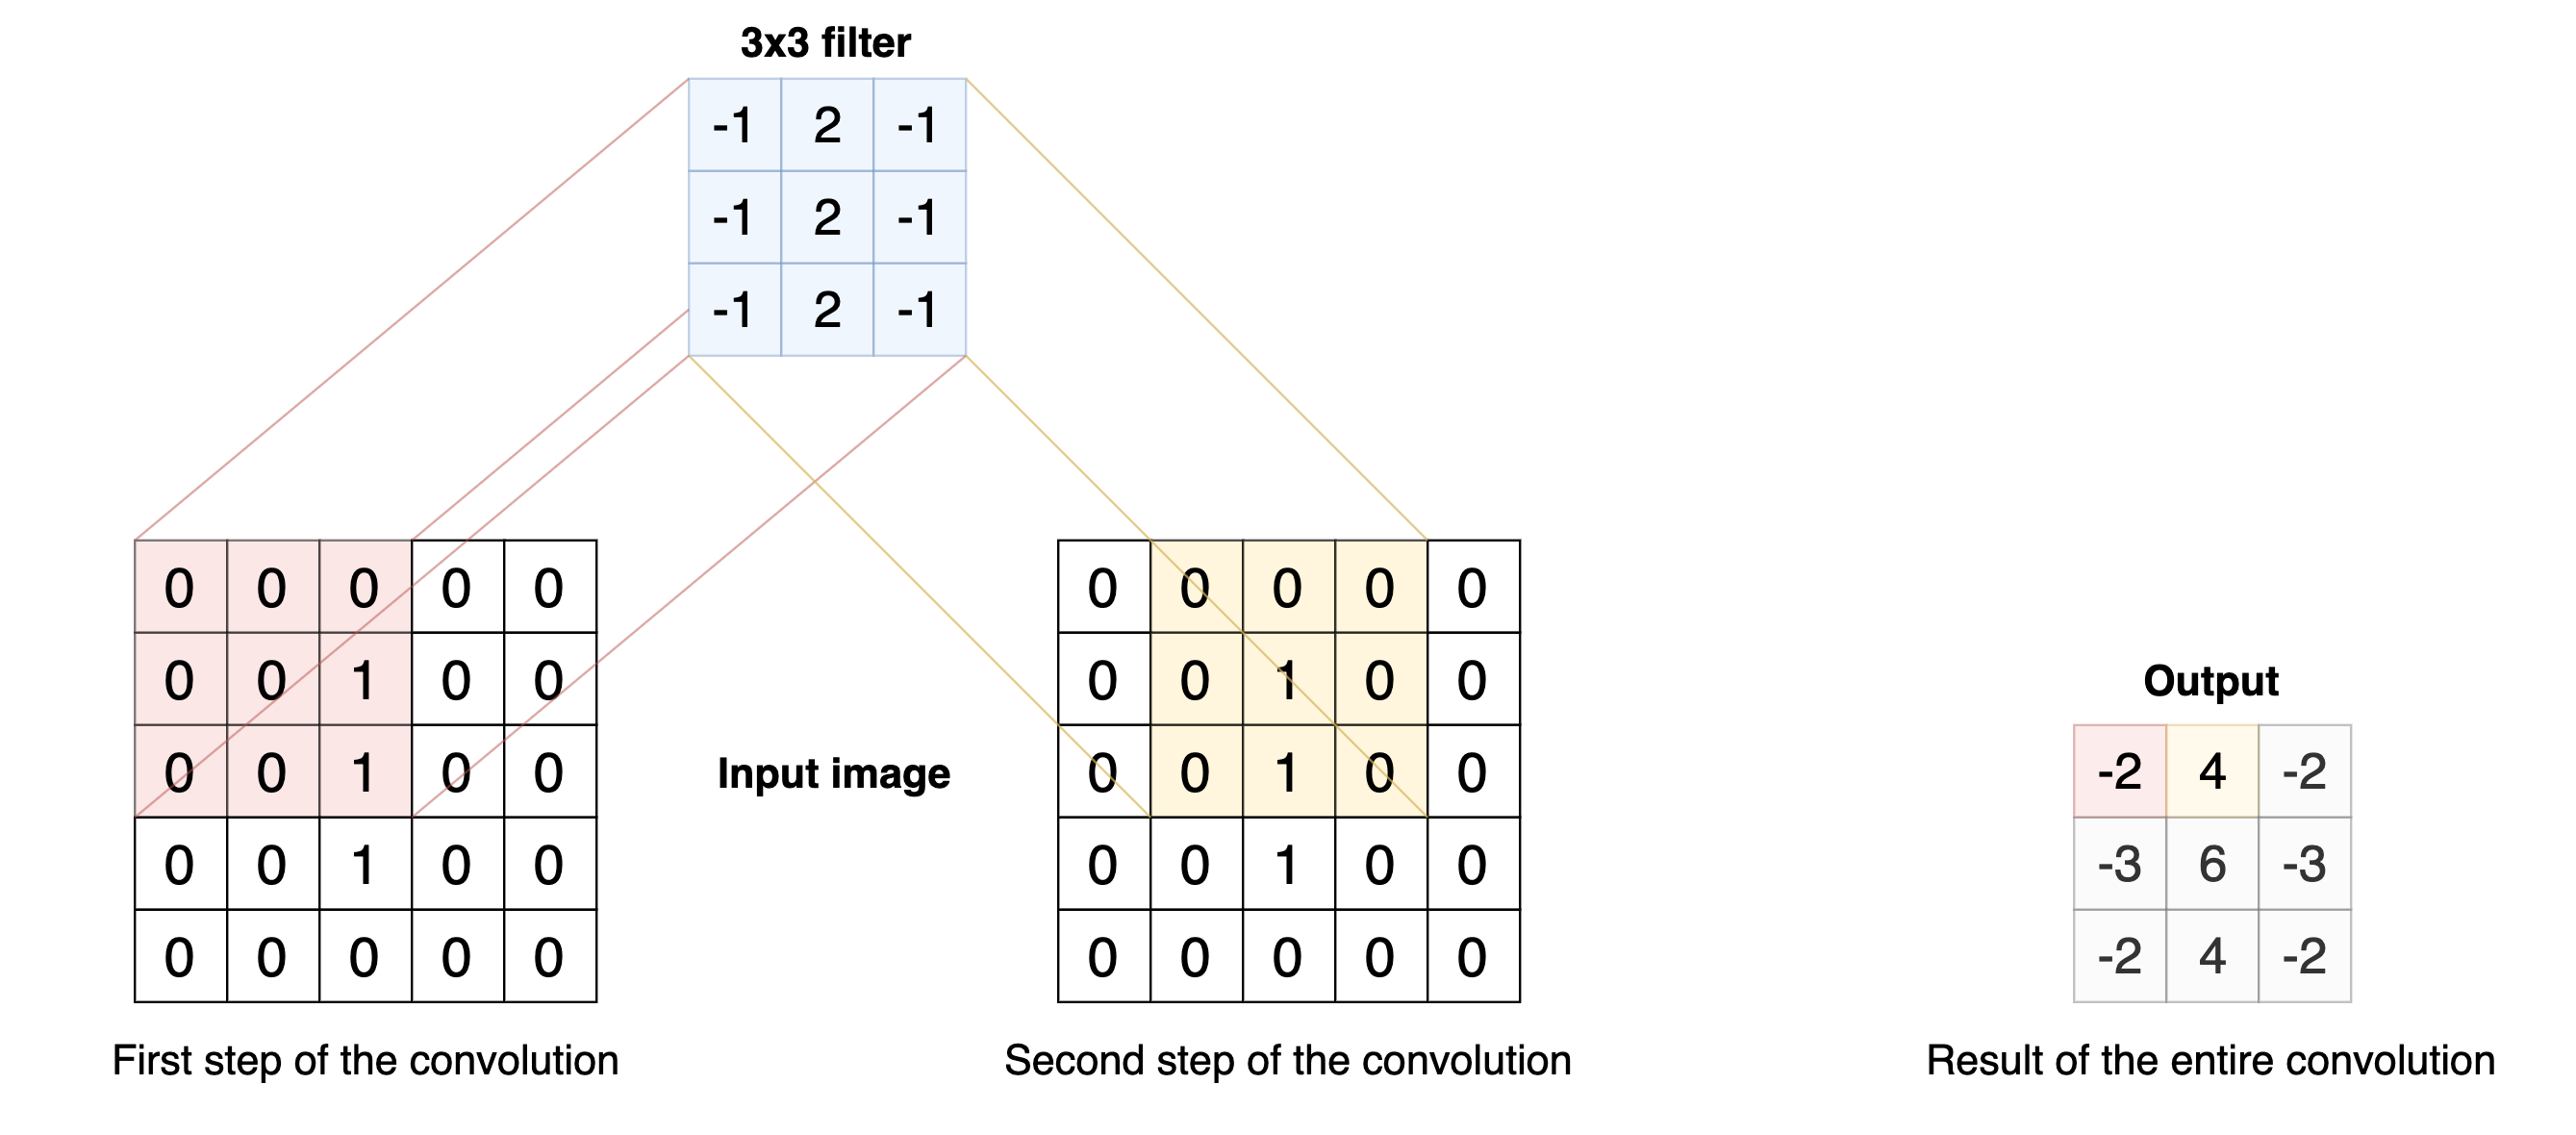
\includegraphics[width=1\textwidth, keepaspectratio=true]{./figures/convolution.png}
\caption{Convolutions - Basic convolution in a CNN}
\label{fig:convolution}
\end{figure}

Different parameters can change the way a convolution behaves. First of all, the previous example relied on a filter moving by respectively one cell to the right and to the bottom. In this case, the so-called "stride" is equal to 1. Other applications could rely on a bigger stride. Furthermore, the previous example reduced the output size of $3x3$ in proportion to the initial input size of $5x5$. To influence the output size, a padding can be added to the outside of the input image, usually filled with 0s. Three ways of padding images are commonly used as shown on figure \ref{fig:convolution_padding}:
\begin{itemize}
	\item \textbf{Valid:} the input image is not padded. This means that the filter only goes through existing pixel values, which makes the output size smaller than the input size. 
	
	\item \textbf{Same:} the input image is padded in a way that makes the output size the same as the input size.
	
	\item \textbf{Full:} the input image is padded so that, in the first step of the convolution, only the bottom-right cell of the filter overlays the pixel value of the image, the rest overlaying padding cells. This makes the output size larger than the input size. 
\end{itemize}

\begin{figure}[!h]
\centering
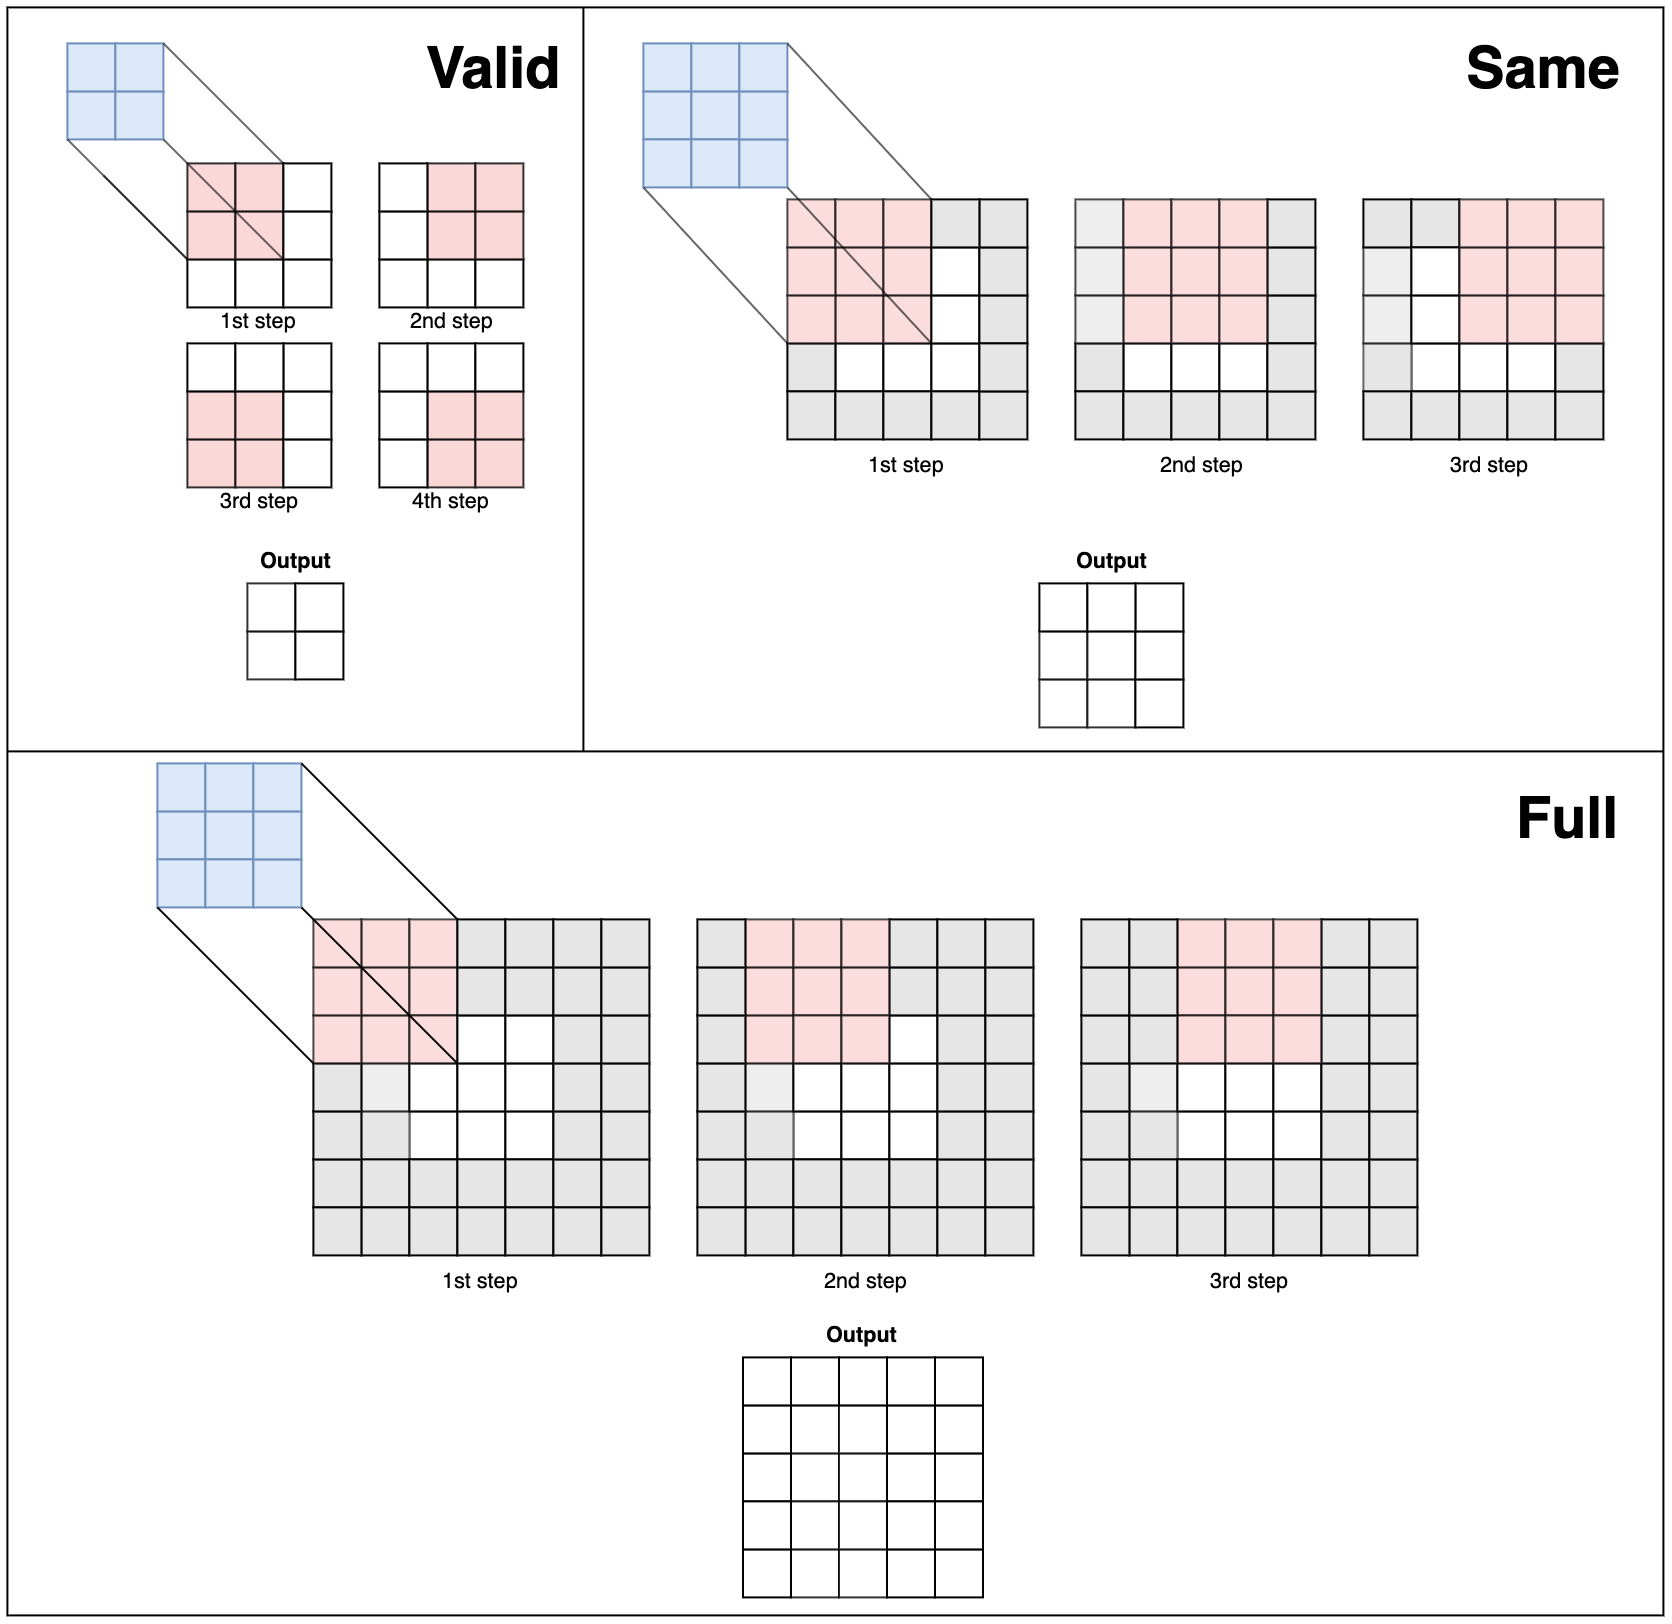
\includegraphics[width=1\textwidth, keepaspectratio=true]{./figures/convolution_padding.png}
\caption{Convolutions - Different padding methods}
\label{fig:convolution_padding}
\end{figure}



\section{Transfer learning}

According to Jason Brownlee, "transfer learning is a machine learning method where a model developed for a task is reused as the starting point for a model on a second task" \cite{30}. The model dedicated to the second task uses some or all parts of the first model (i.e. keeps the same weights and architecture or a part of them) and is then retrained on data available for this task. The first model can either be implemented from scratch if enough data is available or it can simply be downloaded from institutions that release large pretrained models for similar tasks.\\
There are three major benefits \cite{30}:
\begin{itemize}
\item Higher start: the initial skill (before refining the model) on the source model is higher than it otherwise would be.
\item Higher slope: the rate of skill improvement during training of the source model is steeper than it otherwise would be.
\item Higher asymptote: the converged skill of the trained model is better than it otherwise would be.
\end{itemize}
Nevertheless, "in general, it is not obvious that there will be a benefit to using transfer learning in the domain until after the model has been developed and evaluated" \cite{30}.


% !TEX root = ../main.tex

\chapter{Medical information}
\label{ch:medical}
\setlength{\marginparwidth}{3cm}\leavevmode \marginnote{\textbf{Julien}}This chapter gives an overview of the basic medical knowledge that is required to apprehend the following chapters smoothly. First of all, some notions about cancer are described in order to understand what it is and which effects it has on the human body. Second, medical data has its own file formats. To make use of them in a deep learning project, medical files must be processed in a certain way, depending on each format. In fact, formats represent 2D, 3D or even 4D data. Some of them require specific normalization in order to get the right rendering. Finally, some visualization tools were developed to display raw medical files easily. 


\section{Cancer}
\subsection{Basics}
\setlength{\marginparwidth}{3cm}\leavevmode \marginnote{\textbf{Julien}}An accumulation of cells forming a mass is called a tumor. These tumors are detectable thanks to medical imaging (see section \ref{sec:medical_imaging}) and other symptoms. However, not every tumor is as dangerous as the other, as it can be benign (does not contain cancerous cells) or malignant (contains cancerous cells).

The term cancer refers to different phenomena which involve mutation, abnormal multiplication and spreading of cells. As stated by Hanahan et al. in "The Hallmarks of Cancer" \cite{19} and "The Hallmarks of Cancer: The Next Generation" \cite{20}, every malignant tumor acquires six different capabilities during its evolution: 
\begin{itemize}
	\item \textbf{"Sustaining proliferative signaling"}\\ Cancerous cells don't wait for the body's approval to grow and proliferate, contrary to normal cells. They become responsible for their own multiplication.
	\item \textbf{"Evading growth suppressors"}\\
The body sends signals to contain cell growth within a tissue. Cancerous cells are insensitive to these. 
	\item \textbf{"Activating invasion and metastasis"}\\
Metastases are cells whose role is to propagate to other parts of the body in order to colonize and create new tumors. 
	\item \textbf{"Enabling replicative immortality"}\\
Healthy cells replication is limited to a certain amount, which is not the case for cancerous cells. 
	\item \textbf{"Inducing angiogenesis"}
\\Angiogenesis is the process of creating new blood vessels. Tumors have an influence on angiogenesis around them, since they need vascularization to continue growing. 
	\item \textbf{"Resisting cell death"}
\\Apoptosis is the programmed death of cells, which is part of the continuous regeneration of every cell within a body. Cancerous cells survive this programmed death. 
\end{itemize}


\subsection{Seriousness}
\setlength{\marginparwidth}{3cm}\leavevmode \marginnote{\textbf{Julien}}Most cancers can be staged thanks to the TNM system. The T corresponds to the tumor size and its location; the N corresponds to whether or not the tumor has spread to draining lymph nodes; the M corresponds to the presence or absence of metastases in other parts of the body \cite{21}. These pieces of information are used to classify cancer between four (I to IV) or sometimes five (0 to IV) different stages, reflecting the progression and the seriousness of the illness \cite{22}. The earlier they are detected, the higher the chances of recovery are. This aspect makes cancer detection critical since every misjudgment can threaten someone's life. 


\section{Types of medical imaging}
\label{sec:medical_imaging}
\setlength{\marginparwidth}{3cm}\leavevmode \marginnote{\textbf{Julien}}Multiple types of medical imaging exist. The most commonly used to detect cancer are Magnetic Resonance Imaging (MRI), CT (Computed Tomography) scans
%, PET (Positron Emission Tomography) scans
and mammograms. 

MRI relies on magnetic fields to provide a three-dimensional view of body parts, which allows to see the generated images as a volume. Different settings, usually called sequences, make the look of the output vary, as shown on figure \ref{fig:PROSTATEx-t2-adc-dwi}.
Unlike MRI, CT is based on X-rays instead of magnetic fields, but still provides a three-dimensional representation of a body part. Figure \ref{fig:visualize_lung_dcm} shows a lung CT scan.

\begin{figure}[!h]
\centering
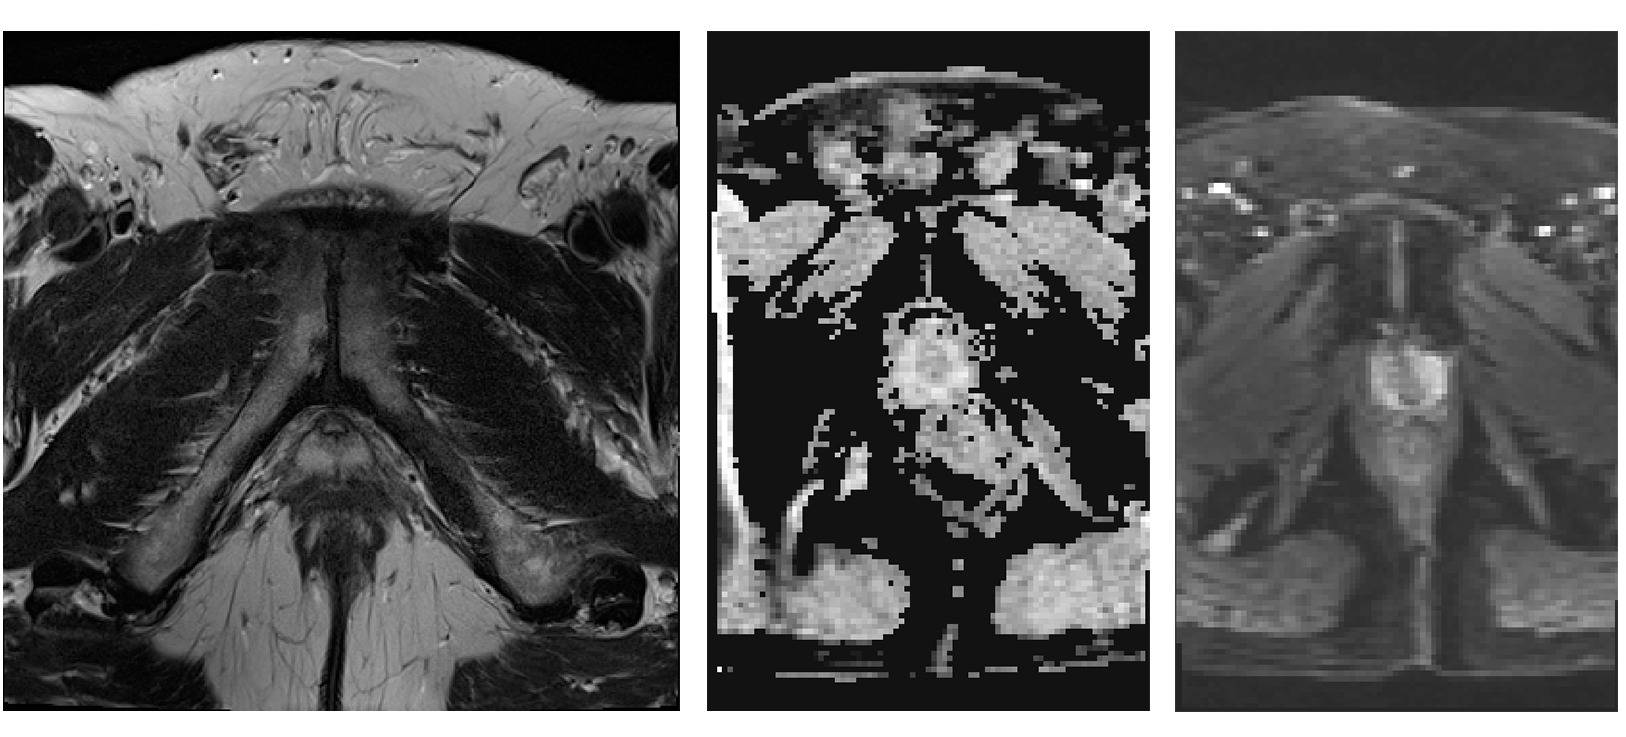
\includegraphics[width=1\textwidth, keepaspectratio=true]{./figures/PROSTATEx-t2-adc-dwi.png}
\caption{MRI - PROSTATEx - From left to right: T2-weighted, ADC and DWI}
\label{fig:PROSTATEx-t2-adc-dwi}
\end{figure}


\section{DICOM file format}
\label{sec:DICOM}
\subsection{Origin}
\setlength{\marginparwidth}{3cm}\leavevmode \marginnote{\textbf{Julien}}The acronym DICOM stands for Digital Imaging and Communications in Medicine. Before the 1980’s, images resulting from CT scans and MRIs were only decodable by machine manufacturers, while the medical community needed to export and share them for other tasks. For that reason, the ACR (American College of Radiology) and the NEMA (National Electrical Manufacturers Association) created a committee to build a standard. After two iterations with other names, DICOM was created in 1993. It standardized the representation of medical images and their transmission since it provided a network protocol built on top of TCP/IP.


\subsection{Data format}
\setlength{\marginparwidth}{3cm}\leavevmode \marginnote{\textbf{Julien}}DICOM files can be viewed as containers of attributes, also called tags. The values of the pixels themselves are stored under the "Pixel Data" tag. Every single DICOM file usually represents a 2-dimensional image, which will form a 3-dimensional volume when put all together. 

Other useful information such as the patient name and ID is directly stored within the DICOM files. This approach aims at linking each image to a specific person and event in order not to mix them up. Each DICOM file can be seen as part of a bigger dataset. 


\subsection{Processing images}
\setlength{\marginparwidth}{3cm}\leavevmode \marginnote{\textbf{Julien}}When manipulating DICOM files, multiple details must be taken into account. 


\subsubsection{Order}
\setlength{\marginparwidth}{3cm}\leavevmode \marginnote{\textbf{Julien}}First of all, the name of the files within datasets is a 6-digit number, from 000000 to the number of images minus one. However, this order doesn’t match the real order of the images. In fact, the correct order is given by the "Instance Number" tags contained in the various files. Therefore, converted images must be sorted by instance number. 


\subsubsection{Data manipulation}
\label{sec:dicom_data_manipulation}
\setlength{\marginparwidth}{3cm}\leavevmode \marginnote{\textbf{Julien}}CT and MRI machines, as well as monitors, differ from one manufacturer to the other and even from one model to the other. DICOM takes this problematic into account by providing specific tags that allow to display the exact same representation of the data, no matter the hardware used. Otherwise, physicians may struggle to detect anomalies because of color and exposition-related variations. 
Therefore, before displaying or converting an image to any format (such as png), pixel data must be normalized. 

The procedure depends on the tags "Window Width" and "Window Center" (one always come with the other). These are used to represent a range of values corresponding to the pixel values in the data. For instance, a window center of 0 and a window width of 200 imply pixel values between -100 and 100. 

If they are missing, a simple conversion is sufficient. The parameters used to convert the data are given by two tags: 
\begin{itemize}
	\item Bits allocated: the number of bits used to represent a single pixel (value: 1 or a multiple of 8)
	\item Samples per pixel: the number of channels for each pixel

\end{itemize}

\noindent Examples: 
\begin{itemize}
\item 1 bit, 1 sample: black and white
\item 8 bits, 1 sample: grayscale
\item 8 bits, 3 samples: RGB
\item 16 bits, 1 sample: grayscale

\end{itemize} 

\noindent If they are included in the DICOM header, a linear transformation must be done to convert the stored representation of the pixels to the correct visualizable one. To do this, two steps are required: 

\begin{enumerate}
	\item \textbf{Apply the Hounsfield correction}\newline
	Hounsfield Units (HU) are used in CT images it is a measure of radio-density, calibrated to distilled water and free air. Provided that the rescale slope and the rescale intercept are included in the DICOM header, the correction is applied thanks to the following formula:
\begin{equation}
	HU = m * P + b
\end{equation}
	where~$m$ is the rescale slope,~$P$ the pixel value, ~$b$ the rescale intercept.

	\item \textbf{Apply a linear transformation}\newline
	The result of the first operation then goes through a linear transformation based on the following conditions: 

\begin{equation}\label{eq:dicom1}
\textrm{if } (P \leq c - 0.5 - \frac{w-1}{2}) \textrm{, then }y = y_{min}
\end{equation}

\begin{equation}\label{eq:dicom2}
\textrm{else if } (P > c - 0.5 + \frac{w-1}{2}) \textrm{, then }y = y_{max}
\end{equation}

\begin{equation}\label{eq:dicom3}
\textrm{else } y = (\frac{P - (c - 0.5)}{w-1}) + 0.5) * (y_{max} - y_{min}) + y_{min}
\end{equation}

where~$c$ is the window center,~$w$ window width, ~$P$ the pixel input value, ~$y$ the pixel output value, ~$y_{min}$ the minimal value of the output range (usually 0), ~$y_{max}$ the maximal value of the output range (usually 255). Equations \ref{eq:dicom1}, \ref{eq:dicom2} and \ref{eq:dicom3} ensure that the pixel values are correctly distributed within the output range. 
\end{enumerate}


\section{NIfTI file format}
\subsection{Origin}
\setlength{\marginparwidth}{3cm}\leavevmode \marginnote{\textbf{Julien}}The Neuroimaging Informatics Technology Initiative (NIfTI) file format is the successor of the ANALYZE file format. The main problem of the latter was that it was lacking information about orientation in space. Therefore, the interpretation of stored data could be problematic and inconsistent. For instance, there was a real confusion to determine the left and right sides of brain images. Hence, the NIfTI file format was defined to overcome this major issue.


\subsection{Data format}
\setlength{\marginparwidth}{3cm}\leavevmode \marginnote{\textbf{Julien}}Unlike the ANALYZE format that used two files to store the metadata and the actual data, the NIfTI file format stores them in one single file “.nii” but keeps this split between the real data and the header for compatibility. This has the advantage to facilitate the use of the data and avoid storing the data without the meta-data. The NIfTI format can also be compressed/decompressed on-the-fly using the “deflate”  algorithm.


\subsection{Overview of the header structure}
\setlength{\marginparwidth}{3cm}\leavevmode \marginnote{\textbf{Julien}}With the goal of preserving the compatibility between the ANALYZE and the NIfTI formats, both headers have the same size of 348 bytes. M. Winkler confirms this fact by claiming "some fields were reused, some were preserved, but ignored, and some were entirely overwritten"~\cite{52}. Details about the different fields contained in the header can be found in the reference of the previous citation.


\section{RAW and MHD file formats}
\setlength{\marginparwidth}{3cm}\leavevmode \marginnote{\textbf{Julien}}Some datasets use a combination of RAW and MHD files. The latter contain metainformation about their corresponding RAW file(s) which contain the data. In most cases, each MHD file points to a unique RAW file whose name is the same as the MHD file name. A single RAW file can be used to represent three-dimensional data, i.e. the combination of multiple two-dimensional images. Libraries such as \mbox{SimpleITK} in Python allow to manipulate RAW images in an easy way. 



\section{Visualization tools}
\setlength{\marginparwidth}{3cm}\leavevmode \marginnote{\textbf{Julien}}
Processing data manually increases the probability of making mistakes. For that matter, visualization tools relying on the same processing code as the ones used to generate training images were developed. Their primary goal is to compare our visual representation of an image to the one obtained in professional pieces of software. These tools are convenient to visualize a dataset easily. In some cases (especially RAW/MHD images), no free software capable of reading the files was available, which made the corresponding tool useful. 


\subsection{DICOM}
\setlength{\marginparwidth}{3cm}\leavevmode \marginnote{\textbf{Julien}}Visualizing DICOM files is pretty straightforward since each file represents a single two-dimensional image. However, a lot of pixel transformations and normalizations have to be applied to obtain the desired result (see section \ref{sec:dicom_data_manipulation}), which may be a source of errors. Our tools allows to display a single DICOM file as well as a sequence of files if the function is fed with a directory. Users can then scroll through the Z-axis, displaying the next or previous slice. 

\begin{figure}[!h]
\centering
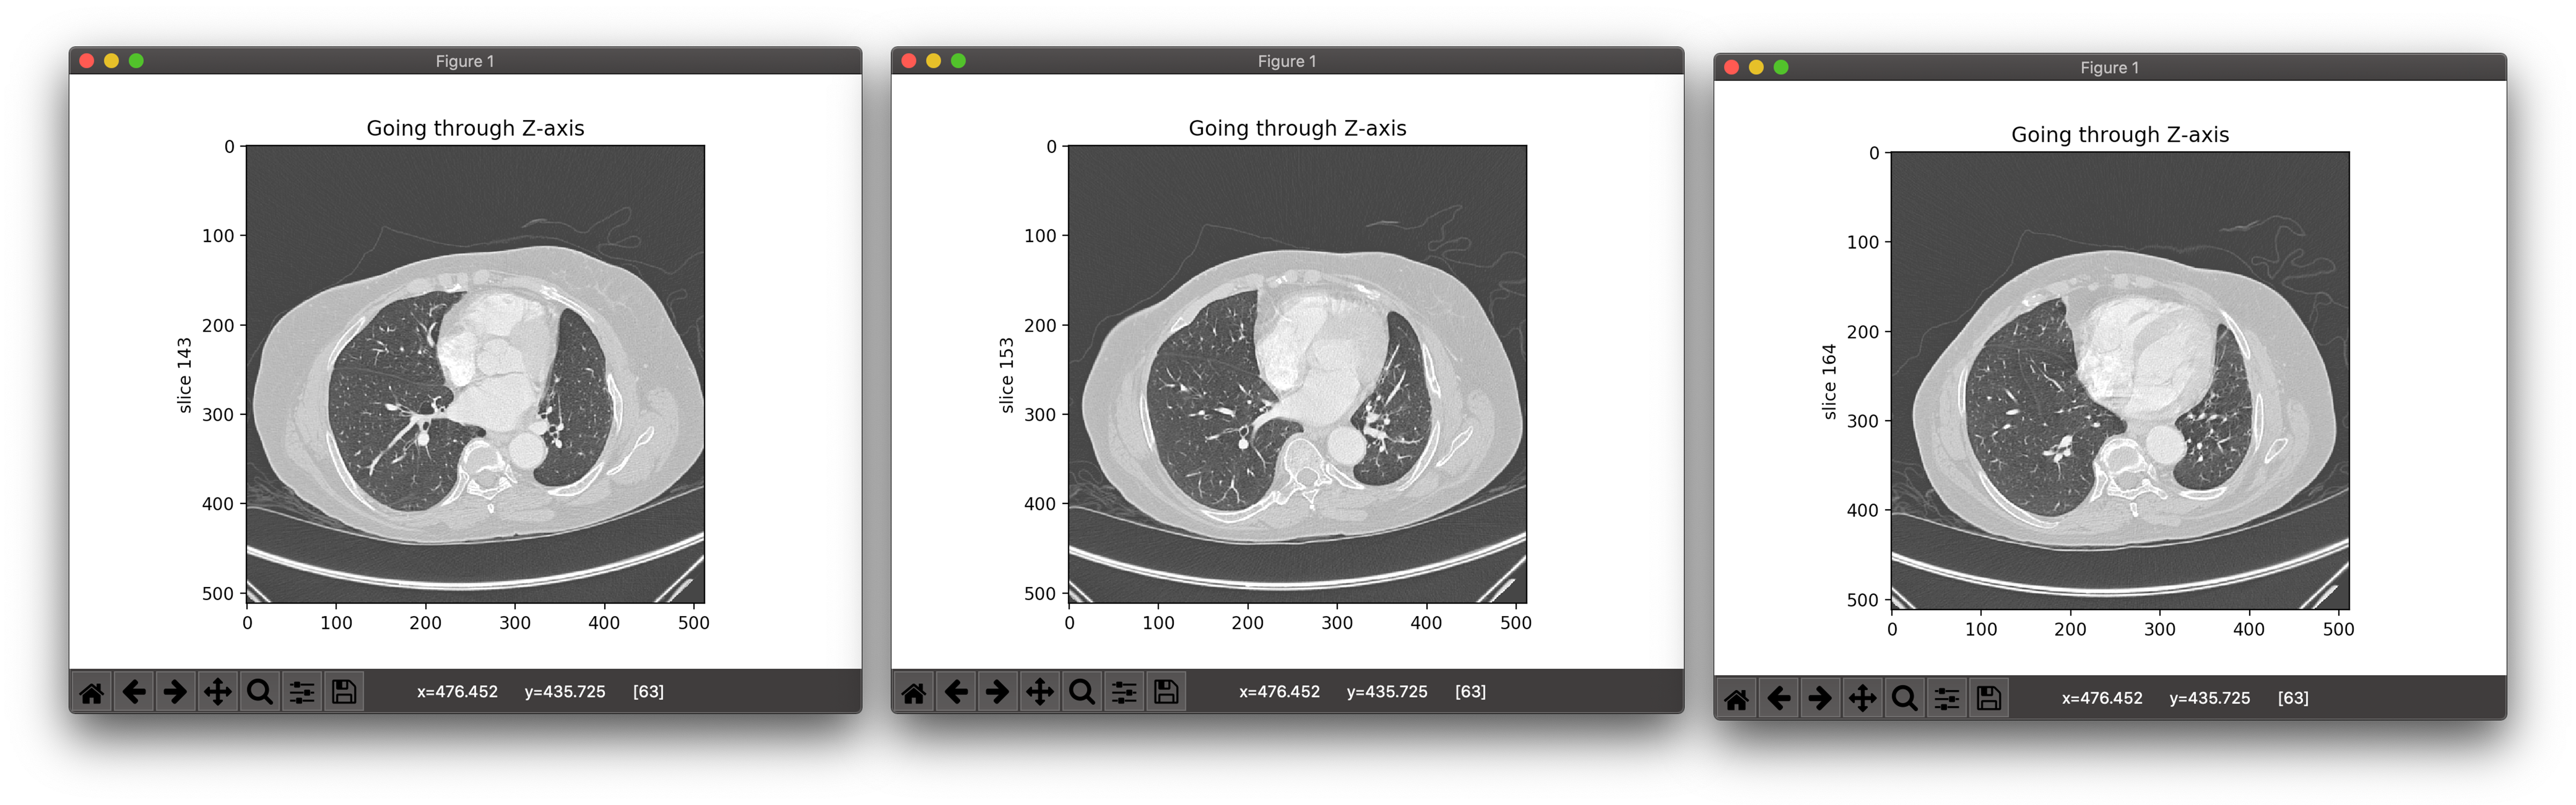
\includegraphics[width=\textwidth, keepaspectratio=true]{./figures/visualize_lung_dcm.png}
\caption{Visualization of a folder of DICOM files}
\label{fig:visualize_lung_dcm}
\end{figure}


\subsection{NIfTI}
\setlength{\marginparwidth}{3cm}\leavevmode \marginnote{\textbf{Julien}}As a single NIfTI file can contain three- or four-dimensional data (the fourth dimension being time), our visualization tool takes this aspect into consideration by allowing to scroll through them: scrolling with the mouse goes through slices belonging to a specific timestamp over a specific axis, while the left and right arrows allows to jump to the same slice at another timestamp. When reaching the end of a timestamp with the mouse, the first slice of the next timestamp is displayed. Furthermore, the three-dimensionality implies that the volume is viewable from three different perspectives. For example, a three-dimensional brain volume can display it from the top of the head to the bottom, from one ear to the other and from the back of the head to the person's face. Therefore, the user can choose a specific axis to navigate through. If no axis is chosen, all three perspectives are shown one after the other.

\begin{figure}[!h]
\centering
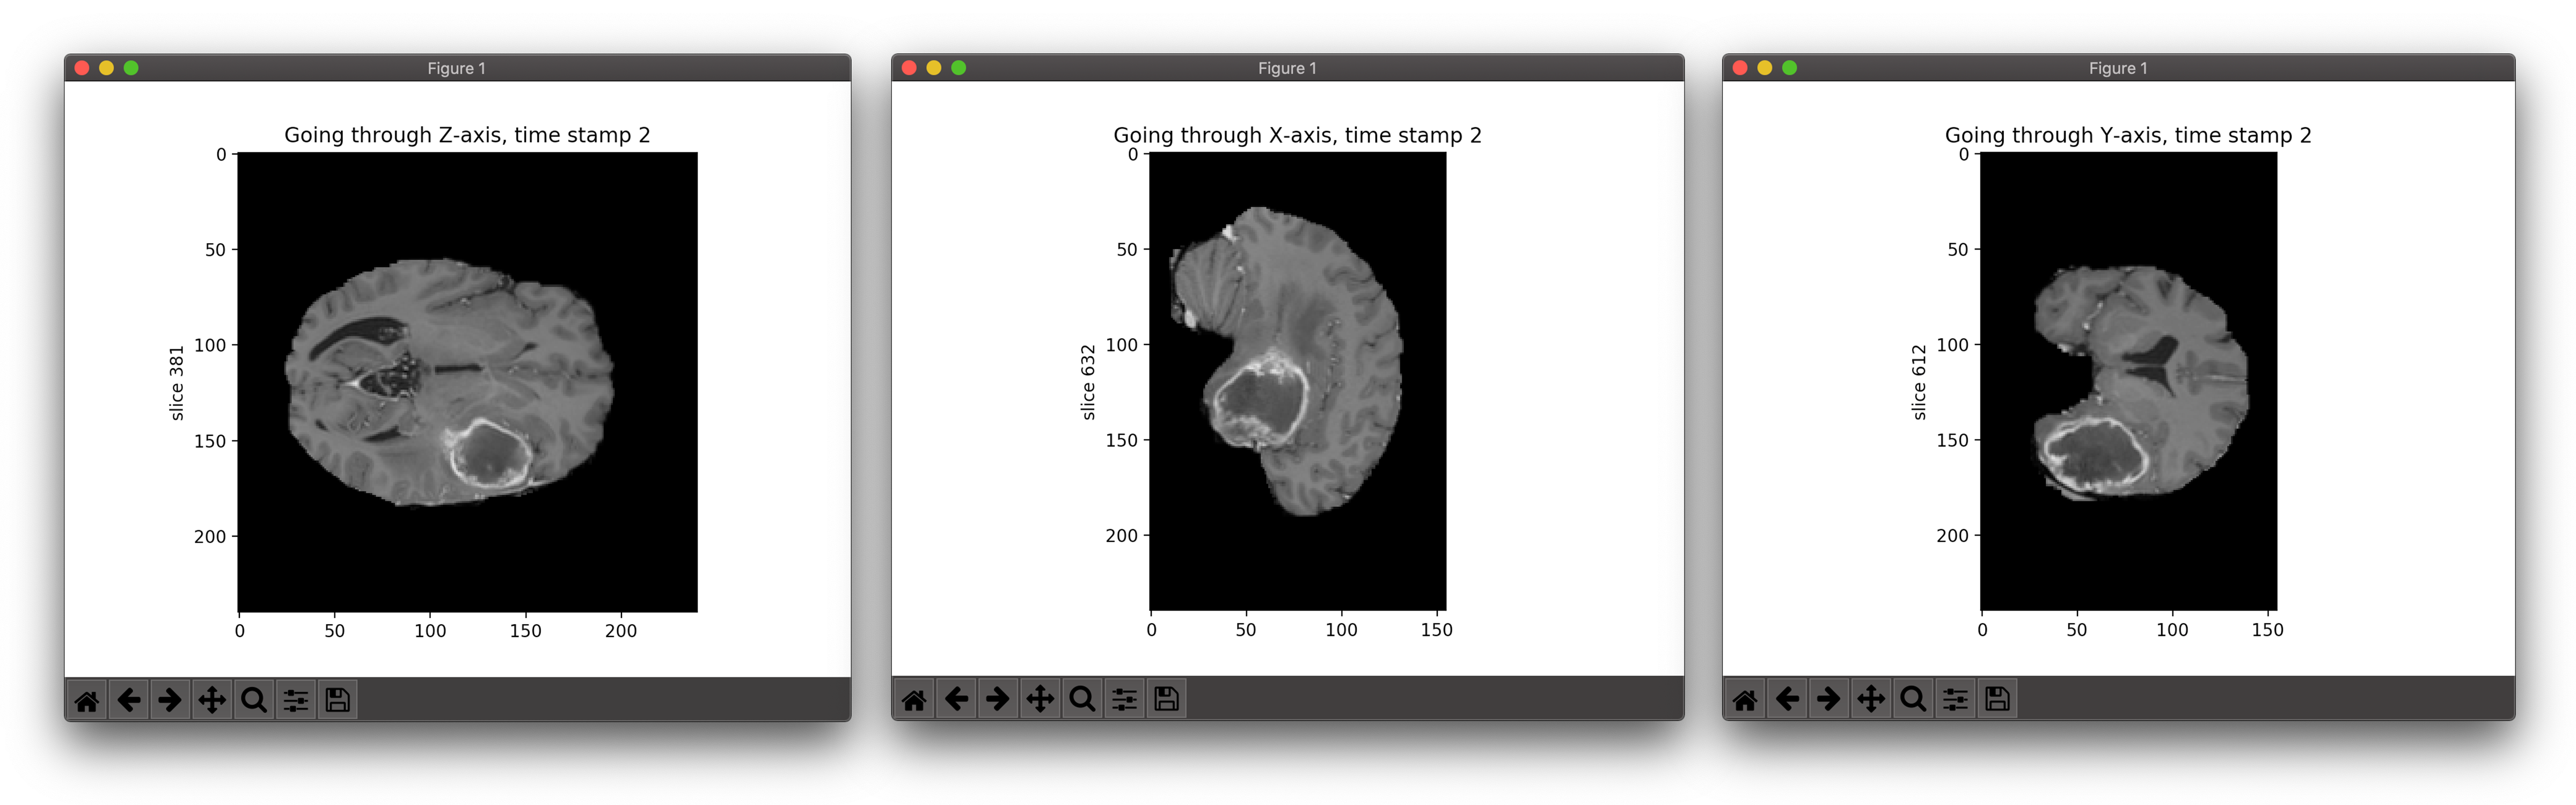
\includegraphics[width=\textwidth, keepaspectratio=true]{./figures/visualize_brain_nii.png}
\caption{Visualization of a four-dimensional NIfTI file}
\label{fig:visualize_brain_nii}
\end{figure}


\subsection{RAW}
\setlength{\marginparwidth}{3cm}\leavevmode \marginnote{\textbf{Julien}}Medical RAW files are three-dimensional, which means that a single file contains a volume, i.e. a succession of 2D slices. Scrolling with the mouse goes through slices over a specific axis. Like the NIfTI file format, the user can profit from the three-dimensionality by displaying the body part from three different perspectives. This tool was particularly useful since no free software capable of handling these files was available. Photography-related programs such as Photoshop can open RAW pictures but not these three-dimensional ones. 

\begin{figure}[!h]
\centering
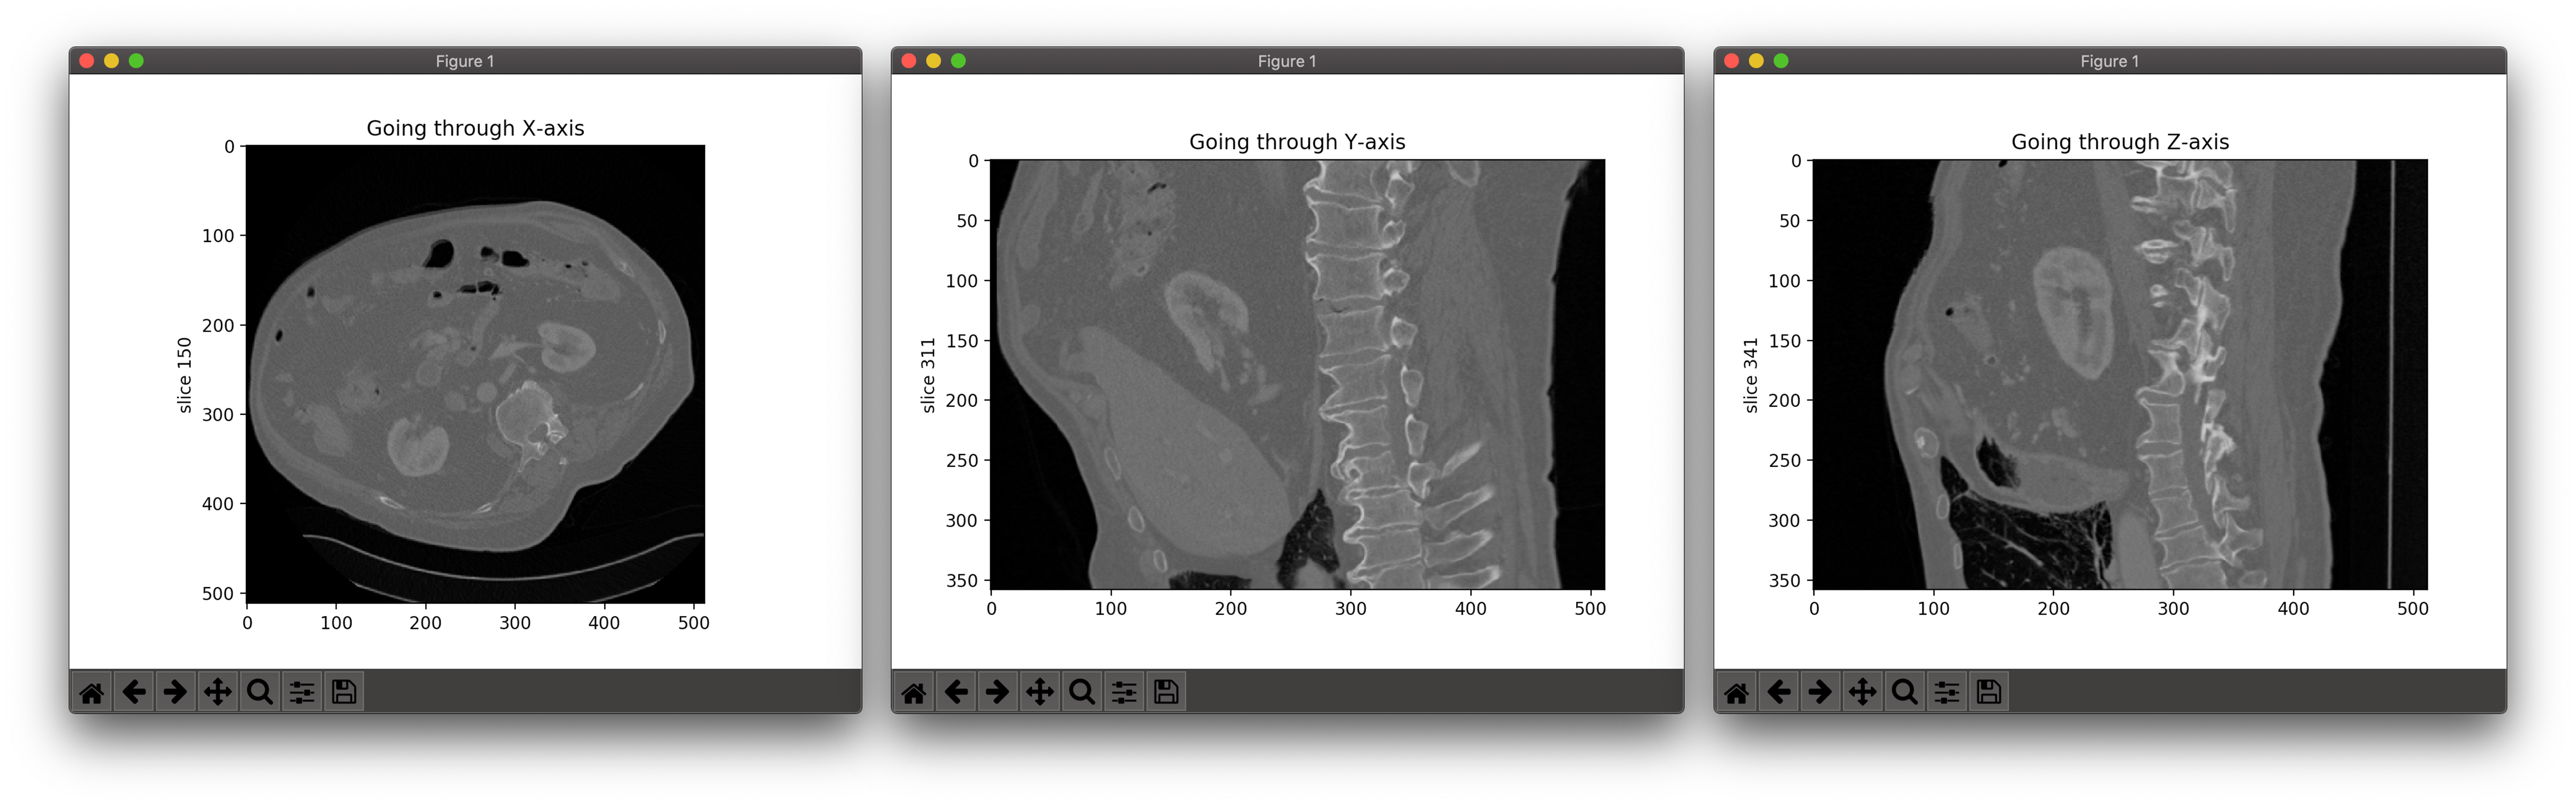
\includegraphics[width=\textwidth, keepaspectratio=true]{./figures/visualize_liver_raw.png}
\caption{Visualization of a three-dimensional RAW file}
\label{fig:visualize_liver_raw}
\end{figure}


\section{Conversion to PNG}
\setlength{\marginparwidth}{3cm}\leavevmode \marginnote{\textbf{Julien}}In addition to the visualization tools, libraries allowing to convert medical files into PNG files were developped. The main one is called "anydatasettopng" and is the one to use to convert any file format to PNG since it makes use of the others. Given a root directory, it scans the latter and its subdirectories to find all DICOM, NIfTI and RAW/MHD files. Then, each file is converted to PNG and saved into the same directory as the one it came from. This library allows to keep an easily accessible visual representation of medical files without having to rely on a specific piece of software to display them. Finally, it also played the role of debugging tool since the conversion techniques are the same as the ones used further in this work. 


\subsection{8-bit conversion}
\setlength{\marginparwidth}{3cm}\leavevmode \marginnote{\textbf{Julien}}Medical data is often represented over 16 bits. However, exporting images to PNG require 8-bit images. To transpose a 16-bit image to an 8-bit one, the procedure described by algorithm \ref{alg:16_to_8_bits_conversion} was applied. 

\begin{algorithm}
    \caption{16 to 8 bits conversion}
    \label{alg:16_to_8_bits_conversion}
    \begin{algorithmic}[1] % The number tells where the line numbering should start
        \Procedure{16\_to\_8\_bits\_conversion}{$pixel\_array$}
        		\State{$Pixel_{min} \gets$ minimal pixel value in $pixel\_array$}
        		\State{$Pixel_{max} \gets$ maximal pixel value in $pixel\_array$}
        		\For{$pixel\_value$ in $pixel\_array$}
        			\State $pixel\_value \gets \frac{(pixel\_value - Pixel_{min}) * 255.0}{Pixel_{max} - Pixel_{min}}$
        		\EndFor
        		\State Modify object type to 8 bits
        		\State Export $pixel\_array$ to PNG
        \EndProcedure
    \end{algorithmic}
\end{algorithm}
% !TEX root = ../main.tex

\chapter{Approach}
\label{ch:approach}

What we do: improve cancer detection/classification on medical imaging
How we do it: transfer learning

\section{Improving cancer classification/detection}


\section{Process overview}

Find data -> Process data -> Verify data processing (visualization, comparing NumPy arrays and PNGs, etc.) -> Train 
% !TEX root = ../main.tex

\chapter{Data processing}
\label{ch:data_processing}

\section{DICOM file format}

\subsection{Origin}

The acronym DICOM stands for Digital Imaging and Communications in Medicine. Before the 1980’s, images resulting from CT scans and MRIs were only decodable by machine manufacturers, while the medical community needed to export and share them for other tasks. For that reason, the ACR (American College of Radiology) and the NEMA (National Electrical Manufacturers Association) created a committee to build a standard. After two iterations with other names, DICOM was created in 1993. It standardized the representation of medical images and their transmission since it provided a network protocol built on top of TCP/IP.


\subsection{Data format}

DICOM files can be viewed as containers of attributes, also called tags. The values of the pixels themselves are stored under the "Pixel Data" tag. Every single DICOM file usually represents a 2-dimensional image, which will form a 3-dimensional volume when put all together. 

Other useful information such as the patient name and ID is directly stored within the DICOM files. This approach aims at linking each image to a specific person and event in order not to mix them up. Each DICOM file can be seen as part of a bigger dataset. 


\subsection{Processing images}

When manipulating DICOM files, multiple details must be taken into account. 

\subsubsection{Order}
First of all, the name of the files within datasets is a 6-digit number, from 000000 to the number of images minus one. However, this order doesn’t match the real order of the images. In fact, the correct order is given by the "Instance Number" tags contained in the various files. Therefore, converted images must be sorted by instance number. 

\subsubsection{Data manipulation}
\label{sec:data_manipulation}
CT and MRI machines, as well as monitors, differ from one manufacturer to the other and even from one model to the other. DICOM takes this problematic into account by providing specific tags that allow to display the exact same representation of the data, no matter the hardware used. Otherwise, physicians may struggle to detect anomalies because of color and exposition-related variations. 
Therefore, before displaying or converting an image to any format (such as png), pixel data must be normalized. 

The procedure depends on the tags "Window Width" and "Window Center" (one always come with the other). These are used to represent a range of values corresponding to the pixel values in the data. For instance, a window center of 0 and a window width of 200 imply pixel values between -100 and 100. 

If they are missing, a simple conversion is sufficient. The parameters to use to convert the data are given by two tags: 
\begin{itemize}
	\item Bits allocated: the number of bits used to represent a single pixel (value: 1 or a multiple of 8)
	\item Samples per pixel: the number of channels for each pixel

\end{itemize}

\noindent Examples: 
\begin{itemize}
\item 1 bit, 1 sample: black and white
\item 8 bits, 1 sample: grayscale
\item 8 bits, 3 samples: RGB
\item 16 bits, 1 sample: grayscale

\end{itemize} 

\noindent If they are included in the DICOM header, a linear transformation must be done to convert the stored representation of the pixels to the correct visualizable one. To do this, two steps are required: 

\begin{enumerate}
	\item \textbf{Apply the Hounsfield correction}\newline
	Hounsfield Units (HU) are used in CT images it is a measure of radio-density, calibrated to distilled water and free air. Provided that the rescale slope and the rescale intercept are included in the DICOM header, the correction is applied thanks to the following formula:
\begin{equation}
	HU = m * P + b
\end{equation}
	where~$m$ is the rescale slope,~$P$ the pixel value, ~$b$ the rescale intercept.

	\item \textbf{Apply a linear transformation}\newline
	The result of the first operation then goes through a linear transformation based on the following conditions: 

\begin{equation}\label{eq:dicom1}
\textrm{if } (P \leq c - 0.5 - \frac{w-1}{2}) \textrm{, then }y = y_{min}
\end{equation}

\begin{equation}\label{eq:dicom2}
\textrm{else if } (P > c - 0.5 + \frac{w-1}{2}) \textrm{, then }y = y_{max}
\end{equation}

\begin{equation}\label{eq:dicom3}
\textrm{else } y = (\frac{P - (c - 0.5)}{w-1}) + 0.5) * (y_{max} - y_{min}) + y_{min}
\end{equation}

where~$c$ is the window center,~$w$ window width, ~$P$ the pixel input value, ~$y$ the pixel output value, ~$y_{min}$ the minimal value of the output range (usually 0), ~$y_{max}$ the maximal value of the output range (usually 255). Equations \ref{eq:dicom1}, \ref{eq:dicom2} and \ref{eq:dicom3} ensure that the pixel values are correctly distributed within the output range. 

\end{enumerate}


\section{NIfTI file format}

\subsubsection{Origin}
The Neuroimaging Informatics Technology Initiative (NIfTI) file format is the successor of the ANALYZE file format. The main problem of the latter was that it was lacking information about orientation in space. Therefore, the interpretation of stored data could be problematic and inconsistent. For instance, there was a real confusion to determine the left and right sides of brain images. Hence, the NIfTI file format was defined to overcome this major issue.


\subsubsection{Data format}
Unlike the ANALYZE format that used two files to store the metadata and the actual data, the NIfTI file format stores them in one single file “.nii” but keeps this split between the real data and the header for compatibility. This has the advantage to facilitate the use of the data and avoid storing the data without the meta-data. The NIfTI format can also be compressed/decompressed on-the-fly using the “deflate”  algorithm.


\subsubsection{Overview of the header structure}
With the goal of preserving the compatibility between the ANALYZE and the NIfTI formats, both headers have the same size of 348 bytes. “Some fields were reused, some were preserved, but ignored, and some were entirely overwritten”. Details about the different fields contained in the header can be found here: \url{https://brainder.org/2012/09/23/the-nifti-file-format/}


\section{RAW and MHD file formats}

Some datasets use a combination of RAW and MHD files. The latter contain metainformation about their corresponding RAW file(s) which contain the data. In most cases, each MHD file points to a unique RAW file whose name is the same as the MHD file name. A single RAW file can be used to represent three-dimensional data, i.e. the combination of multiple two-dimensional images. Libraries such as \mbox{SimpleITK} in Python allow to manipulate RAW images in an easy way. 


\section{Conversion}

Medical data is often represented over 16 bits. However, exporting images to PNG require 8-bit images. To transpose a 16-bit image to an 8-bit one, the procedure described by algorithm \ref{alg:16_to_8_bits_conversion} was applied.

\begin{algorithm}
    \caption{16 to 8 bits conversion}
    \label{alg:16_to_8_bits_conversion}
    \begin{algorithmic}[1] % The number tells where the line numbering should start
        \Procedure{16\_to\_8\_bits\_conversion}{$pixel\_array$}
        		\State{$Pixel_{min} \gets$ minimal pixel value in $pixel\_array$}
        		\State{$Pixel_{max} \gets$ maximal pixel value in $pixel\_array$}
        		\For{$pixel\_value$ in $pixel\_array$}
        			\State $pixel\_value \gets \frac{(pixel\_value - Pixel_{min}) * 255.0}{Pixel_{max} - Pixel_{min}}$
        		\EndFor
        		\State Modify object type to 8 bits
        		\State Export $pixel\_array$ to PNG
        \EndProcedure
    \end{algorithmic}
\end{algorithm}


\section{Processing flow}

Schema Datasets -> xxx\_preprocessing.py -> create\_dataset.py -> Train/Val


\subsection{PROSTATEx: From DICOM to NumPy arrays}

The PROSTATEx dataset comes with two CSV files for the training set. The first one, \textit{ProstateX-Findings-Train.csv}, lists all findings with their clinical significance. Multiple findings can be associated with the same patient (ProxID). The second one, \textit{ProstateX-Images-Train.csv}, gives information about where to find the right DICOM file for each patient and each finding. Important labels are "ProxID" (patient ID), "fid" (finding ID, from 1 to $\infty$), "ClinSig" (clinical significance, TRUE or FALSE), "DCMSerNumber" (digit before the dash in the folder name containing DICOM files) and "ijk" (position of the lesion: slice number $k$ at coordinates $(i,j)$, $i,j,k \in [0,\infty]$). Both CSV files are complementary to each other. Algorithm \ref{alg:PROSTATEx_preprocessing} describes the steps involved in converting PROSTATEx's DICOM files to NumPy arrays. 

\begin{algorithm}
    \caption{PROSTATEx preprocessing}
    \label{alg:PROSTATEx_preprocessing}
    \begin{algorithmic}[1] % The number tells where the line numbering should start
        \Procedure{main}{$dataset\_folder, findings\_CSV, slices\_CSV, output\_folder$}
        		\State Create output directories: $"output\_folder/True", "output\_folder/False"$\\
        		\State $findings \gets read\_CSV(findings\_CSV)$ \Comment{ProstateX-Findings-Train.csv}
        		\State $slices \gets read\_CSV(slices\_CSV)$ \Comment{ProstateX-Images-Train.csv}
            \State $meta \gets merge(findings, slices)$\Comment{Both CSV files are complementary to each other.}\\
            \For{$row$ in $meta$}
            		\State $patient\_id \gets row["ProxID"]$
            		\State $finding\_id \gets row["fid"]$
            		\State $mri\_type\_number \gets row["DCMSerNumber"]$
            		\State $clinical\_significance \gets row["ClinSig"]$
            		\State $img\_i, img\_j, img\_k \gets row["ijk"]$
            		\State $slice\_number \gets img\_k + 1$ \Comment{CSV indexing in $[0,\infty]$, DICOM in $[1,\infty]$}\\
                \For{$visit\ in\ patient\_id$'s folder}
                		\For{$mri\_type$ in $visit$}
                			\If {$mri\_type$ starts with "$mri\_type\_number$-"}
                				\For{$dicom\_file$ in $mri\_type$}
                					\If {$slice\_number == dicom\_file.InstanceNumber$}
                						\State{$slice \gets normalize\_dicom(dicom\_file)$} \Comment{see section \ref{sec:data_manipulation}}
                						\State{Save $slice$ in $"output\_folder/clinical\_significance"$}
                					\EndIf
                				\EndFor
                			\EndIf
            			\EndFor
            		\EndFor
            \EndFor
        \EndProcedure
    \end{algorithmic}
\end{algorithm}



\subsection{Lung CT Challenge - From DICOM to NumPy arrays}

Lung CT Challenge is composed of two different subdatasets: one is considered as a calibration set (10 patients) and the other as a test set (60 patients). Since labels were provided for both sets and the amount of data is fairly low, they were merged and used as a training set. 

Regarding labelling, two Excel files, \textit{TestSet\_NoduleData\_PublicRelease\_wTruth} and \textit{CalibrationSet\_NoduleData}, contain labels for these images. In order to facilitate label managing, two CSV files were manually created: \textit{TestSet.csv} and \textit{CalibrationSet.csv}.
Contrary to PROSTATEx, more than two labels were used for this dataset. Both "malignant" and "Primary lung cancer" were considered as positive, whereas "benign" and "Benign nodule" as negative. A third label called "Suspicious malignant nodule" appeared two times. Since the diagnosis was not clearly defined for those images, they were not treated and included in the training data in order to avoid any noise. Algorithm \ref{alg:LungCTChallenge_preprocessing} shows the various processing steps.

\begin{algorithm}
    \caption{Lung CT Challenge preprocessing}
    \label{alg:LungCTChallenge_preprocessing}
    \begin{algorithmic}[1] % The number tells where the line numbering should start
        \Procedure{main}{$dataset\_folder, train\_CSV, test\_CSV, output\_folder$}
        		\State Create output directories: $"output\_folder/True", "output\_folder/False"$\\
        		\State $csv\_training \gets read\_CSV(train\_CSV)$ \Comment{CalibrationSet.csv}
        		\State $csv\_test \gets read\_CSV(test\_CSV)$ \Comment{TestSet.csv}
            \State $csv\_concatenated \gets concat(csv\_training, csv\_test)$\Comment{Both CSV files contain similar information about different patients.}\\
            \For{$row$ in $csv\_concatenated$}
            		\State $patient\_id \gets row["Scan\ Number"]$
            		\State $slice\_number \gets row["Nodule\ Center\ Image"]$ \Comment{Value in $[1,\infty]$}
            		\State $finding\_id \gets row["Nodule\ Number"]$
            		\State $clinical\_significance \gets row["Diagnosis"]$\\
            		\If{$clinical\_significance$ == $"malignant"$ or $"Primary\ lung\ cancer"$}
            			\State{$clinical\_significance \gets True$}
            		\ElsIf{$clinical\_significance$ == $"benign"$ or $"Benign\ nodule"$}
            			\State{$clinical\_significance \gets False$}
            		\ElsIf {$"clinical\_significance$ == $"Suspicious\ malignant\ nodule"$}
            			\State{Continue}
            		\EndIf\\
                \For{$visit\ in\ patient\_id$'s folder}
                		\For{$mri\_type$ in $visit$}
                			\For{$dicom\_file$ in $mri\_type$}
                				\If {$slice\_number == dicom\_file.InstanceNumber$}
                					\State{$slice \gets normalize\_dicom(dicom\_file)$} \Comment{see section \ref{sec:data_manipulation}}
                					\State{Save $slice$ in $"output\_folder/clinical\_significance"$}
                				\EndIf
                			\EndFor
            			\EndFor
            		\EndFor
            \EndFor
        \EndProcedure
    \end{algorithmic}
\end{algorithm}


\subsection{NumPy arrays to PNG files}
Exporting to NumPy arrays instead of image files directly has multiple advantages. First of all, converting medical files to NumPy arrays or PNG files takes more time than converting NumPy arrays to image files. Reason for that is that the former requires a lot of operation as well as pixel normalization, whereas the latter is a mere conversion of one format to the other. This makes data more reusable. Then, it facilitates the debugging process by separating the conversion from medical files to PNG files into two different steps. Finally, the same processing script can be used to convert NumPy arrays from any dataset to PNG images, which eases operations such as generating different training-validation splits, augmenting data, etc.

\begin{algorithm}
    \caption{Create dataset - NumPy arrays to PNG conversion, organizing data into training and validation data}
    \label{alg:create_dataset}
    \begin{algorithmic}[1] % The number tells where the line numbering should start
        \Procedure{create\_pngs}{$dataset\_folder, output\_folder, split$}
        		\State Create output directories: $"output\_folder/[Train|Val]/[0|1]"$\\
        		\State $true\_nparrays\_dict \gets \{"patient\_id" : [file\_name\_1, ...]\}$
        		\State $number\_of\_patients\_true \gets len(true\_nparrays\_dict)$
        		\State $number\_of\_training\_patients\_true \gets \lfloor number\_of\_patients\_true * split \rfloor$
        		\State $false\_nparrays\_dict \gets \{"patient\_id" : [file\_name\_1, ...]\}$\\
        		\State $index \gets 0$
        		\For{$patient\_id, file\_names$ in $true\_nparrays\_dict$}
        			\If{$index < number\_of\_training\_patients\_true$} \Comment{Training set, True}
        				\For{$file\_name$ in $file\_names$}
        					\State $image\_array \gets load(file\_name)$
        					\State $image \gets convertArrayToGrayscaleImage(image\_array)$
        					\State Save image to $"output\_folder/Train/1"$
        				\EndFor
        			\Else \Comment{Validation set, True}
        				\For{$file\_name$ in $file\_names$}
        					\State $image\_array \gets load(file\_name)$
        					\State $image \gets convertArrayToGrayscaleImage(image\_array)$
        					\State Save image to $"output\_folder/Val/1"$
        				\EndFor
        			\EndIf
        			\State{$index \gets index + 1$}
        		\EndFor\\
        		\State $number\_of\_training\_patients\_false \gets \lfloor number\_of\_patients\_false * split \rfloor$
        		\State $false\_nparrays\_dict \gets \{"patient\_id" : [file\_name\_1, ...]\}$
        		\State $number\_of\_patients\_false \gets len(false\_nparrays\_dict)$
        		\State $false\_nparrays\_dict \gets \{"patient\_id" : [file\_name\_1, ...]\}$\\
        		\State $index \gets 0$
        		\For{$patient\_id, file\_names$ in $false\_nparrays\_dict$}
        			\If{$index < number\_of\_training\_patients\_false$} \Comment{Training set, False}
        				\For{$file\_name$ in $file\_names$}
        					\State $image\_array \gets load(file\_name)$
        					\State $image \gets convertArrayToGrayscaleImage(image\_array)$
        					\State Save image to $"output\_folder/Train/0"$
        				\EndFor
        			\Else \Comment{Validation set, False}
        				\For{$file\_name$ in $file\_names$}
        					\State $image\_array \gets load(file\_name)$
        					\State $image \gets convertArrayToGrayscaleImage(image\_array)$
        					\State Save image to $"output\_folder/Val/0"$
        				\EndFor
        			\EndIf
        			\State{$index \gets index + 1$}
        		\EndFor
        \EndProcedure
    \end{algorithmic}
\end{algorithm}

Algorithm \ref{alg:create_dataset} describes how data was split and organized in order for PyTorch to make use of it. To do so, they were split by class (True $\equiv$ 1, False $\equiv$ 0) and role (training or validation). Furthermore, data are split by patients and not by slices. In fact, multiple slices are usually assigned to each patient. Instead of considering each slice separately, which allows to divide a single patient's slices into the training and validation folders, they were treated as a whole. To sum up, an 80-20 split between the training and validation data (split argument set to $0.8$) will use 80\% of the patients as training data and 20\% of the patients as validation data, regardless of the number of slices.
% \include{chapters/ ...}
% % !TEX root = ../main.tex

\chapter{Conclusion}
\label{ch:conclusions}

\section{Conclusion}
\setlength{\marginparwidth}{3cm}\leavevmode \marginnote{\textbf{Cl{\'e}ment}}This work presented the process leading to the development of a deep learning system to classify potentially cancerous lesions, as well as strategies to overcome field-related issues such as the lack of data.

The starting point was the reproduction of Song et al.'s experiment~\cite{07}. Reaching good performance in this part despite being able to reproduce every single trick showed that our processing and training methods were working well. This resulted in a solid baseline that was exploited in order to take part in the "SPIE-AAPM-NCI Prostate MR Classification Challenge”, also called PROSTATEx challenge. Various hyperparameters and ways of processing the data were tested in order to reach an AUC of $0.76$ on this challenge. This score would have placed the model at the 15$^th$ position out of 71 submissions at the time of the challenge, which confirms the robustness of the latter.

Then, the work focused on overcoming one of the main issues in deep learning: the lack of data. To achieve this, transfer learning, as well as more common techniques such as data augmentation, were applied. The particularity of our transfer learning implementation is the intermediate frozen steps. During the latter, the first part of the model (the feature extractor) does not update its weights at all, whereas the second part (the decision maker) does. Experiments showed that: XXXXXX RESULTS XXXXXX.

Throughout this thesis, various reusable tools were developed: visualization of medical imaging files, conversion of medical imaging files to PNG, a PyTorch sampler using undersampling, easy-to-use processing scripts for multiple datasets (PROSTATEx, Kaggle Brain, Lung CT Challenge), processing verification tools (red dot images), training verification tools (gradient flow graphs, metrics plots using Tensorboard), an all-in-one training and testing file which can be adapted to new models and datasets, an end-to-end transfer learning pipeline. All these elements can serve as a baseline or as additions to future projects.

xxxxx


\section{Future Work}
\setlength{\marginparwidth}{3cm}\leavevmode \marginnote{\textbf{Jobin \& Cl{\'e}ment}}This work mainly used a single model architecture based on a VGG-16 network. As MRIs are three-dimensional, using three-dimensional convolutions could improve the results. This would also require new processing techniques which would generates volumes instead of two-dimensional images. However, well-labeled classification datasets can be counted on the fingers of one hand. As deep learning models need large amounts of training data, the continuation of the same work is more or less compromised. On the other hand, tumor segmentation has become popular over the last years. Most cancer-related deep learning challenges aim at segmenting tumors in three-dimensional data, which makes such datasets easy to find. Therefore, the experience and methods acquired in this work could be transposed to segmentation tasks, which could even combine segmentation and classification. Another possibility to deal with the small amount of publicly available datasets is to develop partnerships with hospitals in order to have access to their data. Obviously, this raises questions about data confidentiality and ethics regarding how the latter is used. New platforms ensuring their confidentiality, their public sharing and their quality have to be developed with the goal of encouraging hospitals to share them. This would allow to build even more better models and in an easier way.
xxxxxx




%----------------------------------------------------------------------------------------
%	BIBLIOGRAPHY
%----------------------------------------------------------------------------------------
\printbibliography[heading=bibintoc]


%----------------------------------------------------------------------------------------
%   APPENDIX
%----------------------------------------------------------------------------------------
% Rarely required, only if extra material particularly voluminous
% % !TEX root = ../main.tex

\chapter{Frequently Asked Questions} % Main appendix title
\label{ch:appendix}

\section{How do I change the colors of links?}

The color of links can be changed to your liking using:

{\small\verb!\hypersetup{urlcolor=red}!}, or
{\small\verb!\hypersetup{citecolor=green}!}, or
{\small\verb!\hypersetup{allcolor=blue}!}.
\noindent If you want to completely hide the links, you can use:
{\small\verb!\hypersetup{allcolors=.}!}, or even better:
{\small\verb!\hypersetup{hidelinks}!}.
\noindent If you want to have obvious links in the PDF but not the printed text, use:
{\small\verb!\hypersetup{colorlinks=false}!}.



%----------------------------------------------------------------------------------------
\end{document}
% That's all folks
